\setcounter{part}{34}    % Z

\part{Préparation aux oraux} %8

\section{CCINP \& petites mines}

\subsection{Format des épreuves CCINP (ex CCP)}

\textsf{Préparation :} 30'

\textsf{Interrogation :} 30'

\textsf{Format :} 2 exercices $\neq$, académiques ou ouverts

\textsf{Rapport 2022 :}

\textsl{Chaque sujet est constitué de deux exercices, sachant que les deux exercices proposés portent sur des
domaines différents du programme de physique-chimie, et qu'ils peuvent être sous forme classique
(académique) ou sous forme de sujet ouvert.}

\textsl{Le but de la préparation n'est pas forcément de résoudre entièrement les exercices, mais de mettre
au point une stratégie de résolution et de rassembler les éléments du cours nécessaires à leur
résolution.}


\subsection{Format des épreuves de Mines--Télécom}

\textsf{Préparation :} sans

\textsf{Interrogation :} 30'

\textsf{Format :} 2 exercices $\neq$, académiques ou ouverts

\textsf{Rapport 2022 :}

\textsl{Chaque épreuve a une durée de 30 minutes et est sans préparation. Résolution de deux exercices portant sur des parties différentes de votre programme.}

\textsl{L’examinateur évalue la capacité du candidat à : 
    Lire l’énoncé, identifier les grandeurs pertinentes et faire un schéma ;
    Proposer une stratégie pour résoudre le problème, formuler des hypothèses ; 
    Énoncer des lois et vérifier leurs conditions d’application, expliciter des méthodes de calcul ;
    Avoir un regard critique sur un résultat ou une expression littérale (ordre de grandeur, analyse dimensionnelle) ;
    Communiquer à l’oral (clarté de l’expression, vocabulaire scientifique approprié) ;
    Il évalue aussi votre bonne connaissance des cours.
}

\bigskip

\begin{exercise}{Lunette astronomique}{-1}{Spé}
{Optique géométrique}{lelay}

Galilée souhaite observer les cratères de la lune. Pour ce faire, il voudrait disposer d'une lunette astronomique : pour cela, il lui faut assembler aux extrémités d'un tube deux lentilles convergentes en formant un système afocal, c'est-à-dire que le plan focal image de la première lentille (l'objectif) est confondu avec le plan focal objet de la seconde (l'oculaire).

Galilée souhaite obtenir un grossissement de 9, et le tube dont il dispose fait 1m20 de long. 

\textbf{Quelle est la vergence des lentilles que Galilée doit utiliser, et comment doit-il les agencer ?}

\end{exercise}

\begin{solution}
    $G = f_2/f_1$
    
    $L = f_1 + f_2$
    
    donc $FL = (G+1)f_1$
    
    donc $f_1 = 12$~cm et $f_2 = 108$ cm, $\delta = 1/f$
\end{solution}
\begin{exercise}{Lunettes}{-1}{Spé}
{Optique géométrique}{lelay}

M. Griffin et Mme. Dinkley ont besoin de nouvelles lunettes. 

Mme Dinkley est myope et ne peut pas voir net au delà de trois mètres. M. Griffin est hypermétrope et ne voit rien en dessous d'une distance d'un mètre.

\textbf{Comment concevoir des lunettes adaptées pour que chacun de ces deux personnages ait une vue équivalente à celle d'un oeil emmétrope (qui n'a pas besoin de correction) ?}

\end{exercise}

\begin{solution}
On suppose que les lunettes sont accolées et donc les dioptries s'ajoutent.

En notant $a$ la distance cornée-rétine on a la vergence de l'oeil emmetrope accomodant à l'infini : $\delta_e^\infty = 1/a$. Pour l'oeil myope qui voit à une distance $d_m$, on a $\delta_m^\infty = \frac1a + \frac1{d_m}$. Avec la correction $\delta_m^{corr}$, 

$\delta_m^{corr} + \delta_m^\infty = \delta_e^\infty$ i.e. $\delta_m^{corr} = -\frac1{d_m}$ : vergence négative, verres divergents, dioptrie -1/3

Hypermétrope : pour l'oeil emmétrope on voit net à $d_e = 20$ cm : $\delta_e^0 = 1/a + 1/d_e$

l'oeil hypermétrope voit net à $d_h$ : $\delta_h^0 = 1/a + 1/d_h$

$\delta_h^{corr} + \delta_h^0 = \delta_e^0$ i.e. $\delta_h^{corr} = \frac{1}{d_e}-\frac1{d_h}$ : vergence positive, verres convergents, dioptrie 4.
\end{solution}
\begin{exercise}{Cadre tombant}{-1}{Spé}
{Induction,Thermochimie}{lelay}

On considère un cadre métallique de résistance $R$, de largeur $a$ et de hauteur $h$ disposé verticalement dans le plan $yz$. Le point le plus bas du cadre est placé en $z = z_0 > 0$.

Dans l'espace $0 > z > -H$ se trouve un champ magnétique $\vec{B} = B_0\ve_x$ orthogonal au cadre.

À $t=0$ on lâche le cadre, qui tombe sous l'effet de la gravité $g$.

\begin{questions}
    \question En utilisant la loi de Lenz, expliquer ce qu'il se passe lorsque
    \begin{parts}
        \part Le cadre tombe en restant au dessus du champ magnétique
        \part Le cadre entre dans le champ magnétique
        \part Le cadre tombe dans le champ magnétique (en supposant $H > h$)
        \part Le cadre sors du champ magnétique
    \end{parts}
    \question Pour chacun des cas précédents, donner les équations du mouvement puis le temps $t_s$ de sortie du cadre du champ magnétique.
    % \question Faire la même étude pour un cadre...
    % \begin{parts}
    %     \part Carré de côté $a$, incliné de 45 degrés.
    %     \part Circulaire de rayon $a$.
    % \end{parts}
\end{questions}

\end{exercise}


\begin{exercise}{Rail de Laplace}{-1}{Spé}
{Induction}{lelay}

On considère un rail de Laplace : dans un champ $\vec{B} = B_0\ve_z$, une barre conductrice est placée en $x_0 > 0$ dans la direction $y$ perpendiculairement à une paire de rails dirigés selon $Ox$, écartés d'une distance $a$ et reliés en $x = 0$ par une résistance $R$.

\begin{questions}
    \uplevel{On donne à la tige une vitesse initiale $v_0$.}
    \question Trouver les équations régissant ce problème. En déduire le comportement de la barre aux temps longs ainsi que le temps caractéristique d'évolution de la vitesse de la barre.
    \question Même question, mais cette fois-ci le système est placé sur un plan incliné d'angle $\alpha$
    \question Que se passe-t-il si on remplace la résistance $R$ par une bobine d'inductance $L$ ?
\end{questions}

\end{exercise}
\begin{exercise}{Chaudière}{-1}{Spé}
{Thermo, système ouvert}{lelay, centrale, CCP}

On s’intéresse à un système pour chauffer l’eau. On fait rentrer de l’eau à une température $\theta_\text{e} = 30$~$^\circ$C dans un cylindre de rayon $R_\text{min}= 8$~cm creusé dans un plus grand cylindre de fonte de rayon $R_\text{max} = 40$~cm et de longueur $L = 60$~cm. Une source de chaleur (feu de bois par exemple) fournit une puissance thermique $\phi = 20$~kW à la fonte. L’eau circule avec un débit massique $D_\text{m} = 25$~kg/min. On suppose que la température dans la fonte ne varie que selon le rayon $r$.


\paragraph{Questions :}
\begin{questions}
    \question Déterminer la température $\theta_\text{s}$ de l’eau en sortie
    \question Déterminer la température de la fonte en $R_\text{max}$
    \question Comment évolue le système si l’on arrête simultanément la chauffage ($\phi = 0$) et l’arrivée d’eau ($D_\text{m} = 0$) ?
\end{questions}

Données :
\begin{itemize}
    \item Conductivité thermique de la fonte : 36~W/m/K
    \item Capacité thermique massique de la fonte : 0.45~J/g/K
    \item Masse volumique de la fonte : 7800~kg/m$^3$
    \item Température de fusion de la fonte : 1800~$^\circ$C
    \item Capacité thermique massique de l'eau : 4.18~J/g/K
\end{itemize}

\end{exercise}

\begin{solution}
    
\begin{questions}
    \question ThermoD en système ouvert $D_m c_{eau}(\theta_s-\theta_a) = \phi$. On trouve une augmentation de température de 11 degrés : c'est ok, la température d'une douche
    \question Diffusion dans un cylindre, il faut retrouver l'expression du laplacien en cylindrique $\Delta T = \frac1r \partial_r\qty(\frac1r\partial_rT)$. Il faut se mettre en régime permanent et prendre $T(R_{min}) = \theta_s$ par exemple. On trouve une temp ext de l'ordre de 150 degrés
    \question Il faut dire que tout se stabilise à une température $\theta_f$ et écrire le premier principe entre le moment où on coupe et la fin, puis intégrer pour trouver $\theta_f$.
\end{questions}
\end{solution}
% Niveau :      PCSI - PC
% Discipline :  Elec
% Mots clés :   Elec, Ordre 2

\begin{exercise}{Tube fluorescent}{1}{Sup,Spé}
{\'Electrocinétique, Circuits d'ordre 2}{bermu}


Les tubes fluorescents sont un type particulier de lampes électriques qui produisent de la lumière grâce à une décharge électrique.

Ces tubes s'allument quand la tension à leur bornes dépasse une certaine tension d'allumage $U_a$. Un fois allumé, le tube s'éteint quand la tension descend en dessous de $U_e$, la tension d'extinction, comme l'illustre la figure ci-dessous.

\begin{figure}[H]
    \centering
    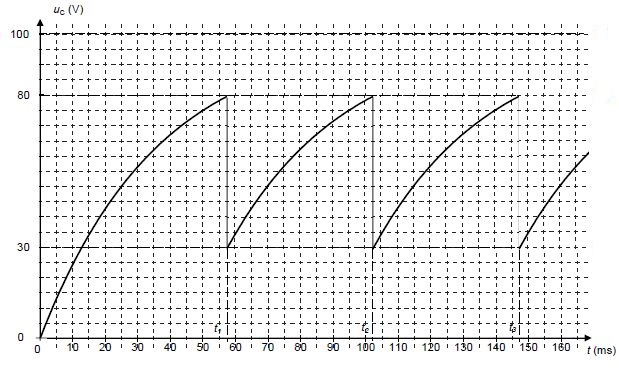
\includegraphics[width=0.65\linewidth]{elec/neon.jpg}
    \caption{Tension au bornes du néon $u_\textsc{c}$ en fonction du temps.}
\end{figure}

\`A $t<0$, le condensateur $C$ est déchargé et le tube est éteint. On allume le générateur à $t=0$.

Le circuit électrique, dans lequel est inséré le tube fluorescent, est schématisé ci-dessous :
\begin{circuit}[Modélisation du tube néon.]
      \draw (0,0)
      to [vsource, v^>=$E$] (0,3)
      to [R, l=$R$] (2,3)
      to [C, l_=$C$, *-*] (2,0)
      to [short] (0,0) {}
      (2,3) to [short] (4,3)
      to [nos, l^=$K$] (4,2)
      to [R, l^=$r$] (4,0)
      to [short] (2,0) {}
      (2.7,0) [open, v_=$u_\textsc{c}$] to (2.7,3) {} ;
      \draw [red, dashed] (3.6,-0.2) rectangle(4.8,3.2) ;
      \node [red] at (4.2,3.5) {Tube néon};
\end{circuit}
Le tube fluorescent est modélisé comme une résistance faible $r$ et un interrupteur $K$ en série. L'interrupteur est ouvert lorsque le tube est éteint et fermé lorsque le tube est allumé.
% Le tube fluorescent est modélisé comme une résistance faible $r$ et un interrupteur $K$ qui s'ouvre et se ferme selon si le tube est allumé ou éteint.

\paragraph{Données :} $E = 100$ V, $R = 60$ k$\Omega$, $r = 10$ $\Omega$, $C = 600$ nF.


\begin{questions}
    \questioncours Condensateurs et dipôles à comportement capacitifs.
    
    \question Décrire le comportement global observé en Fig.~\arabic{exercise}.1 ci-dessus et donner les valeurs de $U_e$ et $U_a$.
    
    \uplevel{On étudie d'abord le circuit entre $t = 0$ et $t_1$.}
    
    \question Simplifier le circuit \arabic{exercise}.1 dans ce cas puis résoudre l'équation différentielle vérifiée par $i$ et $u_\textsc{c}$.
    \question Calculer le temps $t_1$ de l'allumage du néon. Par analogie, quel est le temps $\tau$ du cycle d'allumage du néon ?
    
    \uplevel{On étudie maintenant d'abord le circuit entre $t_1$ et $t_1 + \varepsilon$.}
     
    \question En remarquant que $R\gg r$, simplifier le circuit \arabic{exercise}.1 dans ce cas puis résoudre l'équation différentielle vérifiée par $i$ et $u_\textsc{c}$.
    \question Calculer le temps $t'$ de décharge du condensateur. Justifier que l'on peut négliger ce temps dans le cycle du néon. Voit-on le néon s'allumer et s'éteindre ?
    
\end{questions}
\end{exercise}
\begin{exercise}{Câble coaxial}{-1}{Spé}
{Electromagnétisme,cable coaxial}{mines-T}

On considère deux câbles coaxiaux de rayons respectifs $R_1$ et $R_2 > R_1$. Un gaz isolant occupe tout l'espace entre les deux câbles. On lance une décharge sur le gaz qui le rend conducteur, de conductivité $\gamma$, en supposant qu'il reste à tout instant neutre. A l'instant $t=0$, la câble intérieur porte la charge $q_0$. A l'instant $t>0$, il porte la charge $q(t)$.

\begin{questions}
    \question Calculer $\vec{E}(t)$.
    \question En déduire $\vec{J}(t)$, et $\vec{B}(t)$.
    \question \'Etablir l'équation différentielle vérifiée par $q(t)$, et la résoudre.
\end{questions}

\end{exercise}
% \begin{exercise}{Quantique pas fini}{-1}{Spé}
% {Quantique}{lelay}

% \paragraph{Exercice 1}
% \begin{questions}
%     \question Donner l'expression des niveaux d'énergie $E_n$ d'une particule de masse $m$ dans un puits de potentiel infini de longueur $a$.
%     \question On considère l'atome d'hydrogène, on note $r$ la distance de l'électron au noyau. Calculer $E_n$ sachant que l'électron se trouve dans un puits de potentiel infini de longueur la demi-circonférence de l'atome.
%     \question L'énergie totale de l'électron est $\cal{E}_n$, la somme de $E_n$ et de l'énergie potentielle d'interaction de l'électron avec le noyau. Donner l'expression de $\cal{E}_n$.
%     \question Donner les positions $r_n$ d'équilibre stable de l'électron. Calculer $r_n$ pour $n\in${$1,2,3$}.
%     \question Montrer que $\cal{E}_n$ peut s'écrire sous la forme
%     $$\cal{E}_n=-\dfrac{\text{Ry}}{n^2},$$
%     Ry étant la constante de Rydberg dont on donnera l'expression et la valeur.
%     \question De quelle couleur est la radiation émise par un électron qui passe du niveau d'énergie 3 au 2 ?
% \end{questions}

% \paragraph{Données}
% \begin{itemize}
% \item Masse de l'électron $m = 9,1\times 10^{-31}$ kg ;
%     \item Charge de l'électron $e = 1,6 \times 10^{-19}$ C ;
%     \item Constante de Planck $h = 6,6\times 10^{-34}$ J$\cdot$s ;
%     \item Permittivité du vide $\varepsilon_0 = 8,9 \times 10^{-12}$ H$\cdot$F$^{-1}$.
% \end{itemize}





% \end{exercise}
\begin{exercise}{Décomposition du chlorure de sulfuryle}{-1}{Spé}
{Cinétique}{bermudez}

\begin{flushright}
\noindent\textsl{D'après oral CCINP 2022}
\end{flushright}

On considère la réaction de décomposition du chlorure de sulfuryle
$$\mathrm{SO_2C\ell_{2(g)} \longrightarrow SO_{2(g)} + C\ell_{2(g)}}.$$
Celle-ci a lieu dans une enceinte de volume $V$ et à température $T$ maintenus constants. Les gaz sont supposés parfaits. On note la $p_1$ la pression partielle en SO$_2$C$\ell_2$ et $p$ la pression totale. Initialement, il y a uniquement du $\mathrm{SO_2C\ell_{2(g)}}$ dans l'enceinte et la pression est $p_\text{i}$.

\begin{questions}
    \question Montrer que $p_1 = 2p_\text{i} - p$.
    \question Donner la loi horaire $p(t)$.
    \question \`A l'aide des données, montrez que la cinétique est bien d'ordre 1.
    \question Donner le temps de demi-réaction. Quels sont les facteurs susceptibles de modifier celui-ci ?
    \question Déterminer l'énergie d'activation de cette réaction à l'aide des données.
\end{questions}

\paragraph{Données}~

Pression dans le réacteur $p(t)$ en bar en fonction du temps $t$ pour diverses températures :\\[-2.7em]
\begin{center}
\begin{tabular}{l|llllllllllllll}
\hline
$T$ ($^\circ$C) \textbackslash\  $t$ (s) & 0    & 10   & 20   & 30   & 40   & 50   & 60   & 70   & 80   & 90   & 100  & 130  & 170  & 200  \\ \hline
5                           & 1,00 & 1,08 & 1,06 & 1,07 & 1,12 & 1,19 & 1,18 & 1,25 & 1,28 & 1,25 & 1,28 & 1,33 & 1,49 & 1,50 \\
10                          & 1,00 & 1,06 & 1,06 & 1,14 & 1,24 & 1,28 & 1,26 & 1,27 & 1,29 & 1,35 & 1,37 & 1,50 & 1,62 & 1,64 \\
15                          & 1,00 & 1,12 & 1,14 & 1,19 & 1,27 & 1,33 & 1,34 & 1,37 & 1,42 & 1,50 & 1,53 & 1,67 & 1,71 & 1,79 \\
20                          & 1,00 & 1,09 & 1,25 & 1,34 & 1,36 & 1,39 & 1,47 & 1,50 & 1,61 & 1,65 & 1,72 & 1,76 & 1,83 & 1,87 \\
25                          & 1,00 & 1,20 & 1,28 & 1,35 & 1,50 & 1,55 & 1,66 & 1,72 & 1,79 & 1,80 & 1,84 & 1,88 & 1,96 & 1,93 \\\hline\hline
\end{tabular}
\end{center}
\end{exercise}

\begin{exercise}{Le germanium}{-1}{Spé}
{Cristallographie}{bermudez}

\begin{flushright}
\noindent\textsl{D'après oral CCINP 2022}
\end{flushright}

Une maille de germanium, de paramètre de maille $a = \SI{5,651}{\angstrom}$, a une configuration de type diamant : cubique face centrée dont un site tétraèdrique sur deux est occupé.

\begin{questions}
    \question Calculer la coordinence de la maille et la population.
    \question Calculer la compacité de la maille.
    \question Calculer le paramètre de maille et sa masse volumique.
    \question Peut-on loger un atome d'hydrogène ($r_\text{H} = 53$ pm) dans l'autre site tétrahédrique ? Dans le site octahédrique ?
\end{questions}
   

\paragraph{Donnée :} $M_\text{Ge} = \SI{72,64}{g\cdot mol^{-1}}$.
\end{exercise}

% Niveau :      PCSI *
% Discipline :  Chimie Orga I
% Mots clés :   Spectrométrie UV-visible, Réactions acidobasiques

\begin{exercise}{Raffinage du nickel par le procédé Mond}{-1}{PC,MP}
{Thermochimie, Affinité, Déplacement d'équilibre}{bermu}


    Du nickel de très haute pureté peut être obtenu par l’intermédiaire du nickel carbonyle (tétracarbonylenickel) Ni(CO)$_4$. Ce complexe se forme à température modérée et pression ordinaire par action du monoxyde de carbone gazeux CO$_\text{(g)}$ sur des pastilles de nickel Ni$_\text{(s)}$.
    Aucun autre métal n’est susceptible de réagir dans les mêmes conditions.
    
    Après séparation, le nickel carbonyle est décomposé selon la réaction inverse pour donner du métal de haute pureté.

\begin{questions}
    \question \'Ecrire l'équation de réaction, avec une stoechiométrie 1 pour le nickel.
    \question À l’aide des données thermodynamiques fournies, établir, en fonction de la température $T$, les expressions de l’enthalpie libre standard de la réaction, dans les domaines de température 0--43$^\circ$C et 43--200$^\circ$.
    
Pouvait-on prévoir le signe du coefficient de $T$ dans l’expression de l’enthalpie libre standard de réaction ?

    \question Tracer le graphe de l’enthalpie libre standard de réaction $\Delta_\text{r}G^\circ$ en fonction de la
température $T$.

Quelle est la température d’inversion de l’équilibre ?

    \question Quelle est la variance d’un système à l’équilibre constitué de nickel solide, de monoxyde de carbone et de nickel carbonyle gazeux ? Quel est l’effet sur ce système d’une augmentation de pression à température constante ?
    
    \question Quelle est la variance d’un système à l’équilibre constitué de nickel solide, de monoxyde de carbone et de nickel carbonyle liquide ? Quel est l’effet sur ce système d’une augmentation de température à pression constante ?

    \paragraph{Données :} dans les conditions standard.
    
    \'Ebullition de Ni(CO)$_4$ : $T_\text{vap} = 43$ $^\circ$C, $\Delta_\text{vap}H^\circ = 30$ kJ$\cdot$mol$^{-1}$.
    
    Dans les CNTP :
    \begin{center}
\begin{table}[H]
    \qquad\begin{tabular}{r|cccc}
        Espèce & $\mathrm{Ni_{(s)}}$ & $\mathrm{CO_{(g)}}$ & $\mathrm{Ni(CO)_{4 (\ell)}}$ \\ \hline\hline
        $\Delta_\text{f}H^\circ$ (kJ$\cdot$mol$^{-1}$) & --- & $-111$ & $-632$ \\
        $S_m^\circ$ (J$\cdot$mol$^{-1}\cdot$K$^{-1}$) & $30$ & $198$ & $320$ \\ \hline
    \end{tabular}
\end{table}
    \end{center}
\end{questions}

\end{exercise}


% Niveau :      PCSI *
% Discipline :  Chimie Orga I
% Mots clés :   Spectrométrie UV-visible, Réactions acidobasiques

\begin{exercise}{Oxydation du soufre}{-1}{PC,MP}
{Thermochimie, Affinité, Déplacement d'équilibre}{bermu}

    Nous allons nous intéresser au passage du dioxyde de soufre SO$_{2 \text{(g)}}$ au trioxyde de soufre SO$_{3 \text{(g)}}$ par l'action de l'oxygène O$_{2 \text{(g)}}$. Ce passage se fait essentiellement au contact d’un catalyseur spécifique, le pentaoxyde de vanadium V2O5.

\begin{questions}
    \question \'Ecrire l'équation de réaction, avec une stoechiométrie 1 pour le dioxygène.
    
    \question Calculer son enthalpie standard de réaction et son entropie standard de réaction à $T = 300$ K et en déduire l'expression de l’enthalpie libre standard de réaction pour toute température $T$.
    
    \question Quelle est la température d’inversion de l’équilibre ? Préciser l’expression numérique de $\ln K^\circ(T)$ pour toute température ($K^\circ$ désigne la constante d’équilibre).
    
    \uplevel{Les industriels travaillent vers $T = 430$ $^\circ$C sous $p = P^\circ = 1$ bar avec un léger excès de dioxygène
provenant de l’air par rapport à la quantité stoechiométrique 2 SO$_2$ pour 1 O$_2$. Nous allons interpréter ces choix.}

    \question Partons de $\lambda$ moles de dioxygène pur et de $1 - \lambda$ moles de dioxyde de soufre. Dresser un tableau d’avancement et donner la relation liant à l’équilibre le paramètre $\lambda$, l’avancement $\xi$, la constante d’équilibre $K^\circ$ et la pression totale $p$.
    
    \question À $T$ et $p$ fixées, pour quelle valeur de $\lambda$ a-t-on un avancement $\xi$ maximal ?
    
    \paragraph{Données :} dans les CNTP
    \begin{center}
\begin{table}[H]
    \qquad\begin{tabular}{r|cccc}
        Espèce & $\mathrm{SO_{2 (g)}}$ & $\mathrm{SO_{3 (g)}}$ & $\mathrm{O_{2 (g)}}$ \\ \hline\hline
        $\Delta_\text{f}H^\circ$ (kJ$\cdot$mol$^{-1}$) & $-297$ & $-396$ & --- \\
        $S_m^\circ$ (J$\cdot$mol$^{-1}\cdot$K$^{-1}$) & $248$ & $257$ & $205$ \\ \hline
    \end{tabular}
\end{table}
    \end{center}
\end{questions}

\end{exercise}

\begin{exercise}{Cristallographie du germanium}{-1}{Spé}
{Cristallo}{bermudez}

\begin{questions}

    \question  Donner sa configuration électronique du germanium ($Z = 32$) dans son état fondamental. On rappellera les lois qui permettent de donner cette configuration.
    
    \question On s'intéresse à un oxyde du germanium de formule inconnue Ge$_x$O$_y$. Son cristal est tel que les atomes de germanium suivent un arrangement cubique à face centrées alors que les atomes d'oxygène occupent la moitié des sites tétraédriques.
    Donner les valeurs de $x$ et $y$.

    \question Calculer la masse volumique du cristal.
\end{questions}

\paragraph{Données}
\begin{center}
\begin{tabular}{rcc}
    \hline
     & O & Ge \\
    Rayon atomique (pm) & 60 & 125\\
    Nombre de masse & 16 & 72.6 \\ \hline\hline \\
    Numéro atomique & 8 & 32 \\ \hline\hline 
\end{tabular}
\end{center}

\end{exercise}

\begin{solution}

[Ge] = [Ar] 3d$^{10}$ 4s$^2$ 4p$^2$

CFC population de 4, 8 sites tetraedriques (centre des 8 cubes inscrits) donc GeO : $x=1$ et $y=1$.

\end{solution}
\begin{exercise}{Thermochimie du germanium}{-1}{Spé}
{Thermochimie}{bermudez}

 On s'intéresse désormais à l'équilibre hétérogène à 790 K (en phase gaz et solide) entre GeO$_{\text{ (s)}}$ et H$_{2\text{ (g)}}$ qui produit entre autres du Ge$_\text{(s)}$.
 On dispose initialement de $n$(GeO)$=n_1=1$ mol, $n$(H$_2$)$=n_2=8$ mol, $n$(Ge)$=n_1=1$ mol et $n$(H$_2$O)$=n_1=1$ mol.
 \begin{questions}
    \question Donner l'équation de réaction. De quel type de réaction s'agit-il vis à vis du germanium ?
    \question Déterminer la constante $K^\circ$ de la réaction à $T_0 = 300$ K puis à $T_1 = 790$ K. 
    \question Dans quel sens évolue la réaction ? Déterminer l'état final du système.
\end{questions}

\paragraph{Données}
\begin{center}
\begin{tabular}{rcc}
    \hline
    (à 300 K) & $\mathrm{GeO_{2 (g)} \,/\, Ge_{(s)}}$ & $\mathrm{GeO_{(s)} \,/\, Ge_{(s)}}$ \\
    $E^\circ$ (mV) & $-50$ & $+262$\\ \hline\hline 
\end{tabular}~\\

\medskip


\begin{tabular}{rccccc}
    \hline
    (à 400 K) & Ge$_\text{(s)}$ & $\mathrm{H_2O_{(g)}}$ & $\mathrm{H_{2 (g)}}$ & $\mathrm{GeO_{(g)}}$ & $\mathrm{GeO_{2 (g)}}$ \\
    $S_\text{m}^\circ$ (J$\cdot$mol$^{-1}\cdot$K$^{-1}$) & 168 & 189 & 151 & 111 & 67  \\
    $c_\text{p,m}^\circ$ (J$\cdot$mol$^{-1}\cdot$K$^{-1}$) & 23 & 37 & 29 & 43 & 60\\ \hline\hline 
\end{tabular}\end{center}
\begin{itemize}
    \item $e^\circ = \dfrac{RT}{\scr{F}} \ln10 = 59$ mV à 300 K.
    \item Entropie de vaporisation de l'eau $\Delta_\text{vap}H$(H$_2$O, 300 K)$ = 44$ kJ$\cdot$mol$^{-1}$.
    \item Masse d'un nucléon $m_n = 1,67\times 10^{-27}$ kg.
\end{itemize}

\end{exercise}

\section{Centrale Supélec}
\begin{exercise}{Cuisson des oeufs}{-1}{Spé}
{Thermo}{centrale}

La cuisson des oeufs est un art subtil ancré dans la tradition gastronomique française. De nos jours, les restaurateurs ont des autocuiseurs qui permettent d'avoir une température bien homogène.

Il existe trois principales cuissons des oeufs à l'eau bouillante dans leur coquille 
\begin{itemize}
    \item la cuisson \emph{à la coque}, pour laquelle l'extérieur du blanc est solide, mais pas l'intérieur ni le jaune ;
    \item la cuisson \emph{mollet}, pour laquelle le blanc est solide, mais pas le jaune ;
    \item la cuisson \emph{dure}, pour laquelle le blanc et le jaune sont solides.
\end{itemize}

\`A cela s'ajoute la question sanitaire de l'élimination des salmonelles.

\paragraph{Données :}~\\
L'oeuf peut être considéré en première approximation comme une sphère de rayon $R$ avec :
\begin{itemize}
    \item température de cuisson du blanc : $T_\text{b} = 62^\circ$C ;
    \item température d'élimination des salmonelles : $T_\text{s} = 64^\circ$C pendant 5 minutes ;
    \item température de cuisson du jaune : $T_\text{j} = 68^\circ$C ;
    \item chaleur latente de cuisson des protéines : $L = 1,7$ J$\cdot$kg$^{-1}$ ;
    \item un oeuf d'autruche pèse 1,5 kg environ.
\end{itemize}
Pour les autres données, on pourra considérer que l'oeuf est constitué d'eau liquide.

Pour l'eau :
\begin{itemize}
    \item capacité calorifique de l'eau $c = 4,2$ $\mathrm{J\cdot kg^{-1}\cdot K^{-1}}$ ;
    \item conductivité thermique de l'eau $\lambda = 0,60$ $\mathrm{W\cdot m^{-1}\cdot K^{-1}}$ ;
\end{itemize}

Les réfrigérateurs de la restauration sont généralement maintenus à $T_\text{0} = 4^\circ$C.

\paragraph{Résolution de problème :}~\\
Le restaurateur sort un oeuf du réfrigérateur et le met dans un bain marie maintenu au point d'ébullition de l'eau $T_\text{e}$ (à pression atmosphérique).

\begin{questions}
    \question Représenter qualitativement et à différents instants le profil de température $T(t,r)$ de l'intérieur de l'oeuf.
    \question Par analyse dimensionnelle et avec un bilan énergétique sommaire, évaluer le temps caractéristique $\tau$ de cuisson d'un oeuf dur pour une poule et pour une autruche.
    \question Justifier que l'on puisse négliger l'énergie de solidification des protéines pendant la cuisson.
    \question Retrouver l'équation de la chaleur vérifiée par $T(t,r)$ dans le système de coordonnées adaptées au système. On fera appaitre du temps caractéristique de cuisson $\tau$ dans l'expression et on indiquera les conditions initiales et aux bords vérifiées par $T(t,r)$.
    \question Adimensionner l'équation en introduisant le changement de variable suivant :
        \begin{align*}
            \Theta(s,z) &= \dfrac{T(t,r) - T_\text{e}}{T_\text{0} - T_\text{e}}, &
            z &= r/R, & s = t/T,
        \end{align*}
    \question Trouver l'équation vérifiée par $F(s,z) = z\Theta(s,z)$. Commenter.
%    \question Résoudre cette équation par séparation des variables $F(s,z) = S(s) Z(z)$. Montrer que l'on peut exprimer $\Theta$ sous la forme :
%        $$\Theta(s,z) = \sum_{n=1}^{\infty} \theta_n \dfrac{\sin (n \pi z)}{n \pi z} e^{-n\pi s},$$
%        $\theta_n$ étant des coefficients associés.
%    \question Retrouver les coefficients $\theta_n$ à partir des conditions initiales et donner la solution $T(t,r)$. \\
%        On utilisera que la fonction porte peut s'écrire comme suit :
%        $$\Pi(z) = \left\lbrace \begin{array}{ll}
%            1 & \text{si } -1 < z < 1 \\
%            0 & \text{sinon}
%        \end{array}\right. = -2\sum_{n=1}^{\infty} (-1)^n \dfrac{\sin (n \pi z)}{n \pi z}.$$
%   \question Conclure quant aux différents critères de cuisson de l'oeuf en fonction de $T_\text{e}$ et $T_0$ (considérer $r=0$).
    
\end{questions}

\end{exercise}

%\begin{exercise}{Atmosphère et couche d'Ozone}{-1}{Spé}
{Thermo}{centrale}

\textsl{Extrait adapté de Wikipédia, l'encyclopédie libre.}

\begin{center}\begin{minipage}{.9\textwidth}
L'ozone est un gaz de formule chimique O$_3$. C'est une molécule triatomique dont un des atomes d'oxygène est lié aux deux autres. L'ozone est une variété allotropique de l'oxygène, mais bien moins stable que le dioxygène O$_2$, en lequel il tend naturellement à se décomposer à température ambiante. La rapidité de la réaction dépend de la température, de l'humidité de l'air ou de la présence de catalyseurs.

L'ozone est naturellement présent dans l'atmosphère terrestre, formant dans la stratosphère une couche d'ozone entre 13 et 40 km d'altitude qui intercepte plus de 97 \% des rayons ultraviolets du Soleil, mais est un polluant dans les basses couches de l'atmosphère (la troposphère) où il est toxique pour les être vivants.

\`A 20 km d'altitude, les densités en O$_2$ et en O$_3$ sont respectivement de $4\times 10^{17}$ cm$^{-3}$ et de $2\times 10^{12}$ cm$^{-3}$.
\end{minipage}\end{center}

\paragraph{Données :}~\\
Mécanisme réactionnel du cycle de Chapman de formation et de décomposition de l'ozone :
\begin{align}
    \mathrm{O_3} & \underset{k_{-1}}{\overset{k_1}{\resizebox{4em}{1.5ex}{~$\rightleftharpoons$~}}} \mathrm{O_2 + O^{\bullet\bullet}} \tag{R1} \ \\
    \mathrm{O_2} & \overset{k_2}{\resizebox{4em}{.8ex}{~$\rightarrow$~}} \mathrm{2O^{\bullet\bullet}} \tag{R2}
    \\
    \mathrm{O_3 + O^{\bullet\bullet}} & \overset{k_3}{\resizebox{4em}{.8ex}{~$\rightarrow$~}} \mathrm{2O_2} \tag{R3}
\end{align}
On considérera que les concentrations des gaz et non leur pression partielle pour effectuer les calculs cinétiques et thermodynamiques chimiques.

On peut considérer que la réaction (R1) est un équilibre rapide et que la concentration en [O$^{\bullet\bullet}$] est négligeable devant les autres.

Données thermodynamiques à $300$ K :
\begin{center}\begin{tabular}{l|cc}
    & O$_2$ & O$_3$ \\ \hline
    $\Delta_\text{f}H^\circ$ ($\mathrm{kJ\cdot mol^{-1}}$) & --- & 142,12  \\
    $S_\text{m}$ ($\mathrm{J\cdot mol^{-1}\cdot K^{-1}}$) & 204,82 & 237,42 \\
    Energie de première ionisation (eV) & 12,07 & 12,43 \\ \hline\hline
\end{tabular}\end{center}

\paragraph{Résolution de problème :}~\\
Nous allons dans cet exercice justifier que l’ozone se forme dans les hautes couches de l’atmosphère.

\begin{questions}
    \question Donner la formule de Lewis de l'Ozone.
    \question\textsf{Modèle cinétique :} On appelle [Ox] = [O$^{\bullet\bullet}$] + [O$_3$].  Interpréter cette quantité.
    \question En utilisant les approximations adéquates, montrer que l'équation cinétique des Ox peut s'écrire
    $$\dv{\mathrm{[Ox]}}{t} = 2 k_2 \mathrm{[O_2]} - k\dfrac{\mathrm{[Ox]^2}}{\mathrm{[O_2]^2}},$$
    avec $k$ dont on précisera l'expression. Commenter ce taux en fonction de la température.
    \question\textsf{Modèle thermodynamique :} Quelle est l'équation globale de la transformation de O$_3$ et O$_2$ ? Dans quel cas peut-on considérer que l'on a atteint l'équilibre thermodynamique ?
    \question Le cas échéant, donner une relation entre [O$_3$], [O$_2$] et la température $T$. En déduire la tendance du O$_3$ a être détruit dans la basse atmosphère et produit dans la haute atmosphère.
\end{questions}

\end{exercise}
 HORS PROGRAMME MP
\begin{exercise}{Indétermination d'Heisenberg}{-1}{Spé}
{Quantique}{centrale}

% \textsl{D'après Centrale-Supélec, sujet zero (2015)}

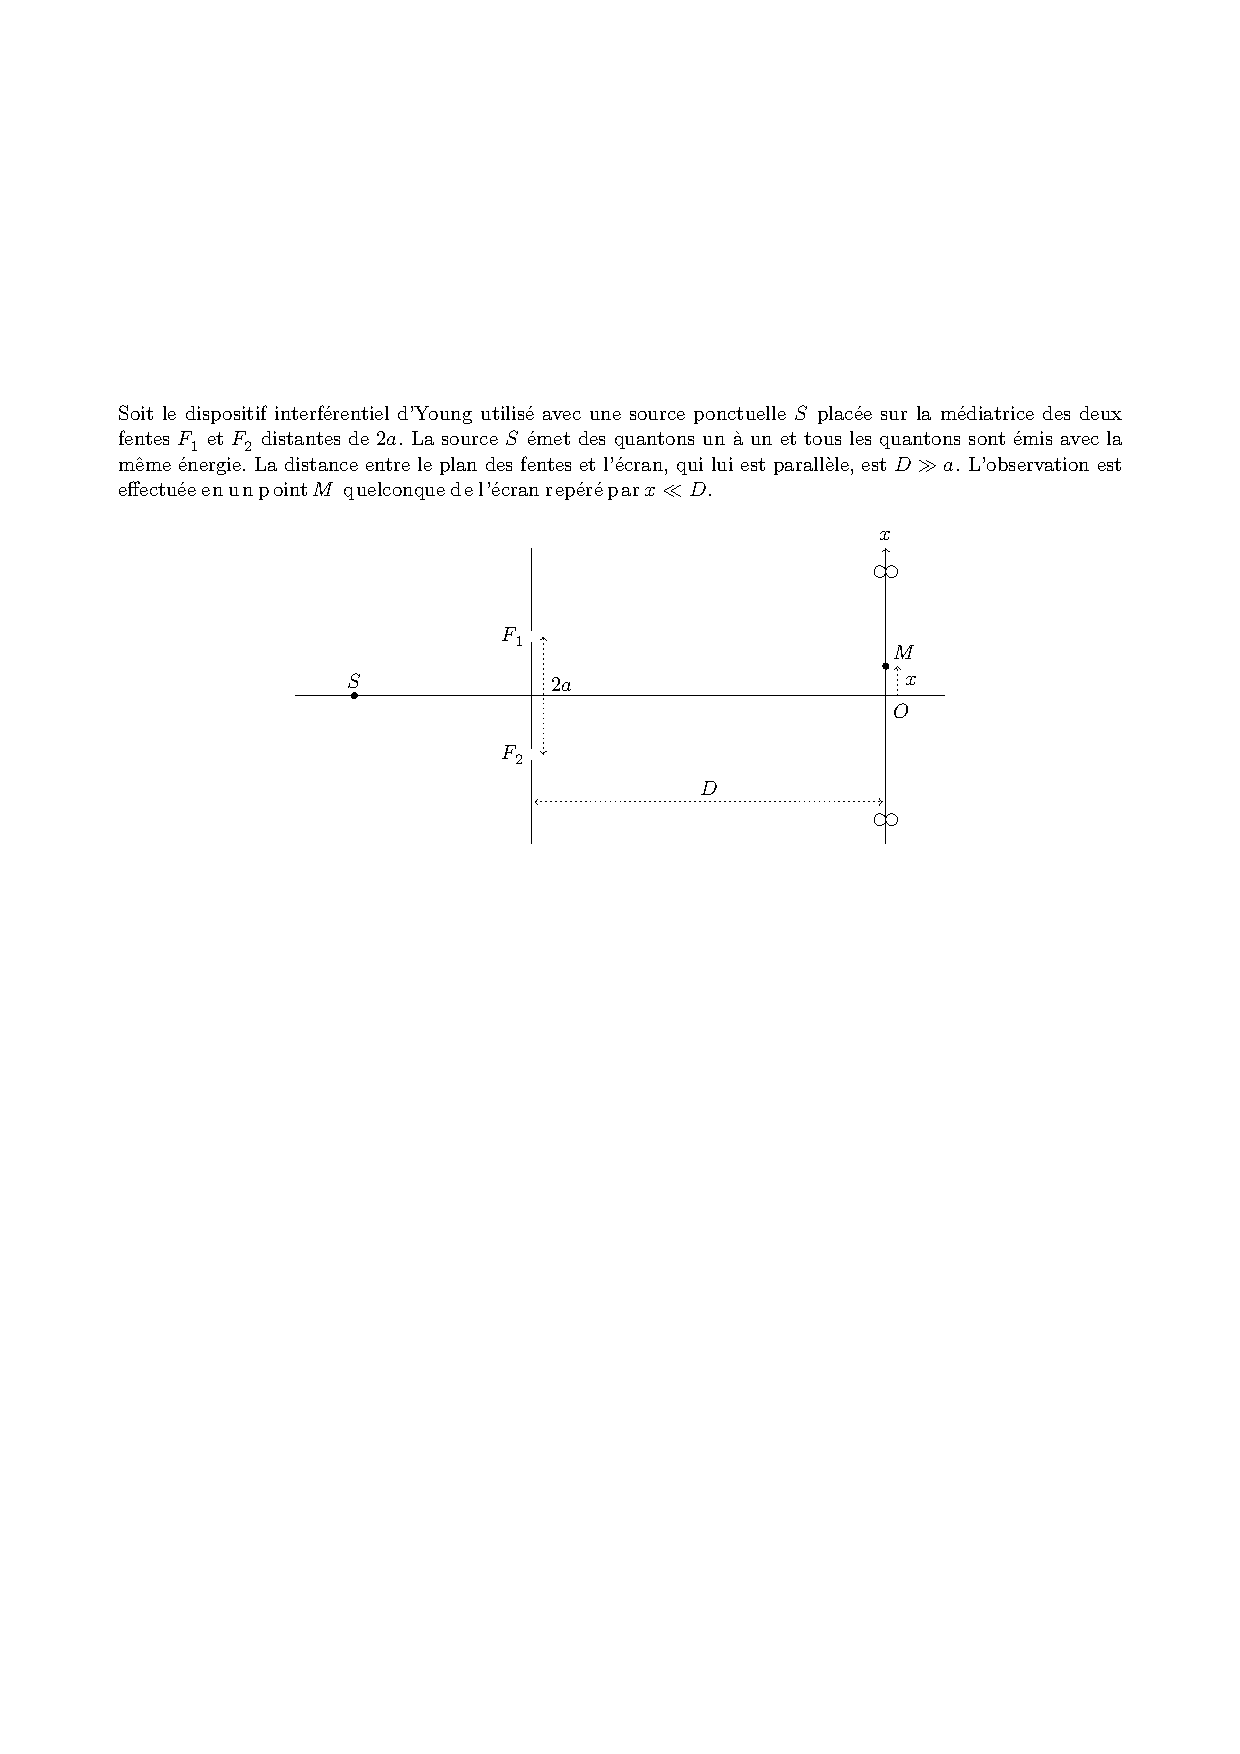
\includegraphics[width=\linewidth]{oraux/centrale/heisenberg1.pdf}

\paragraph{Résolution de problème :}~\\
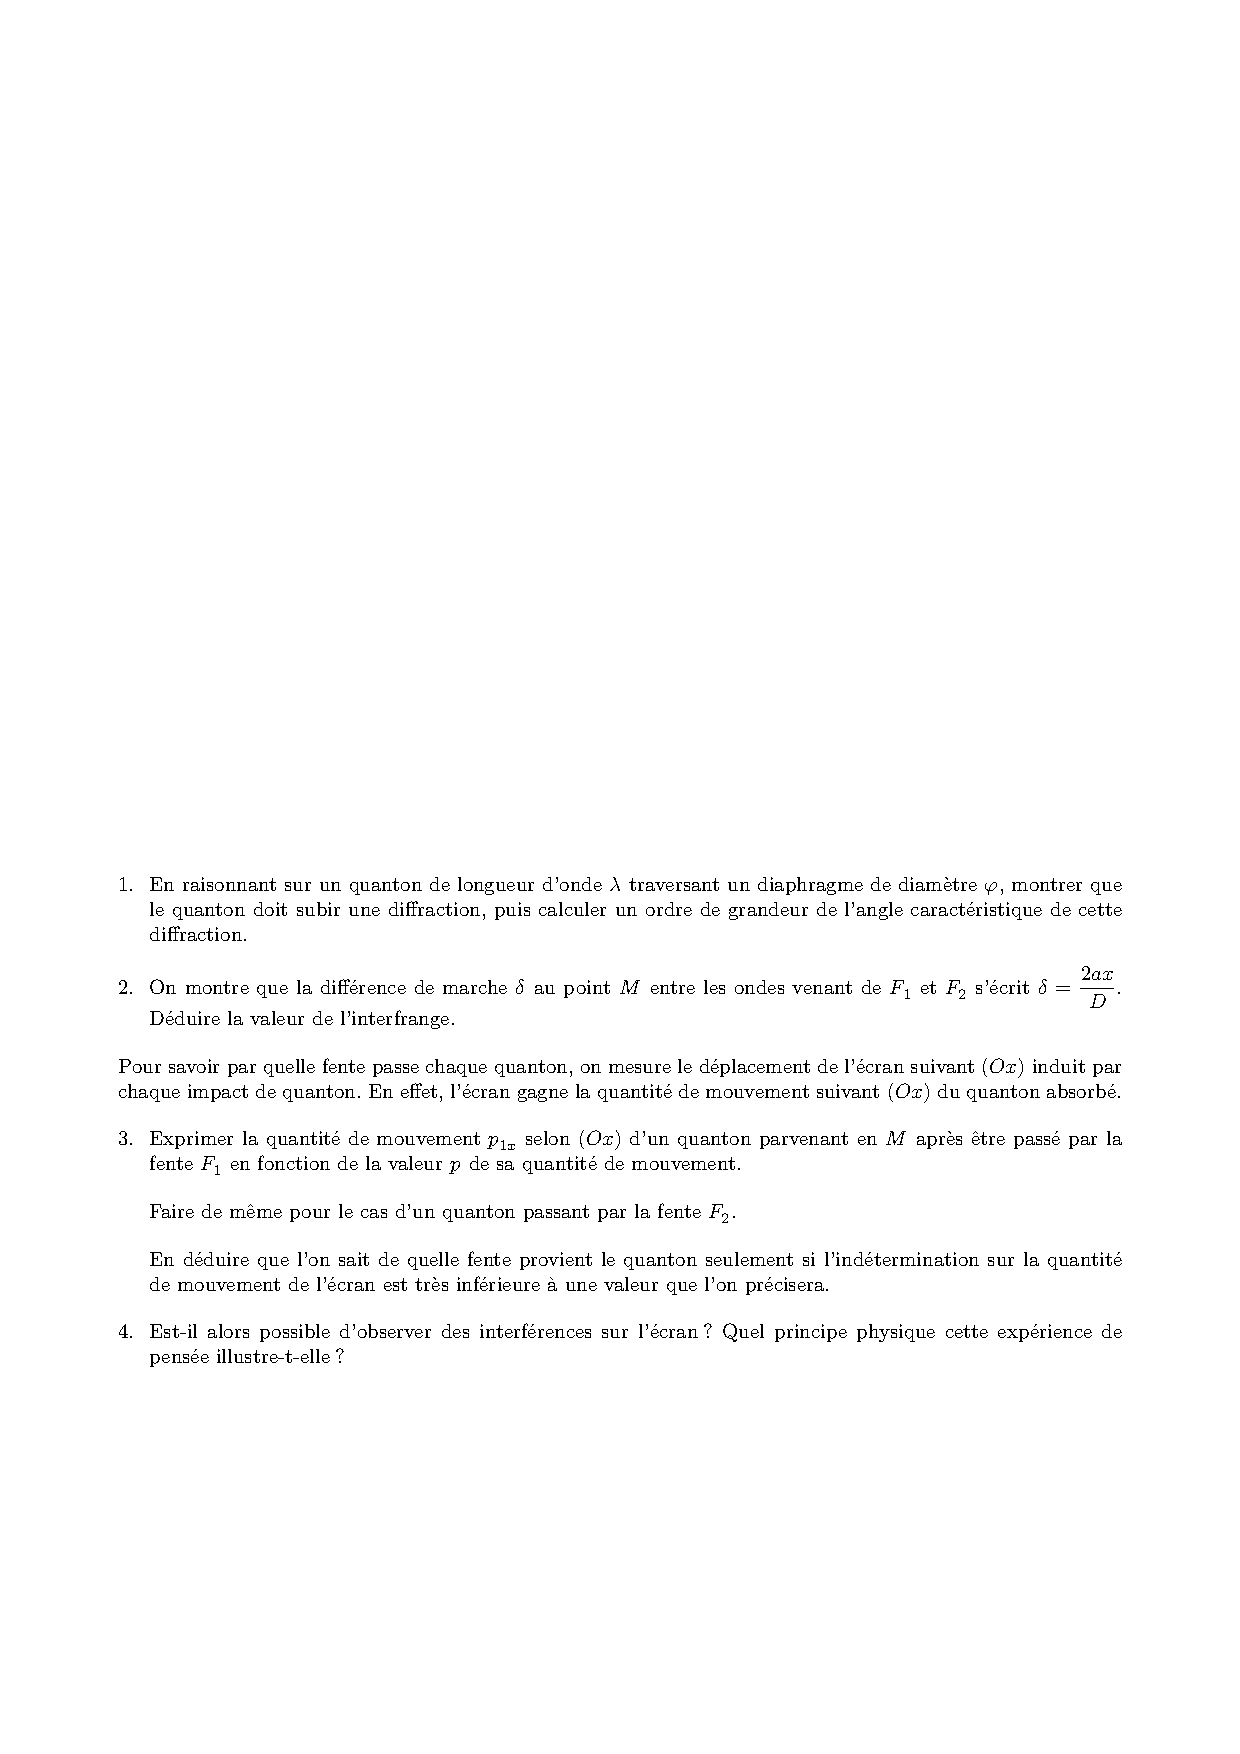
\includegraphics[width=\linewidth]{oraux/centrale/heisenberg2.pdf}

\end{exercise}
\begin{exercise}{Photo aillée}{-1}{Spé}
{Optique géométrique}{lelay, centrale}

Une tête d'ail fait à peu près 7 cm de diamètre. La photographie reproduite ci-dessous a été prise à une distance $D$ de l'ail avec un appareil photographique assimilable à une lentille convergente de distance focale $f' = 50$~mm en utilisant un diaphragme de rayon $R$ et une pellicule de 24x36~mm placée à une distance $d$ de la lentille.

\begin{figure}[H]
    \centering
    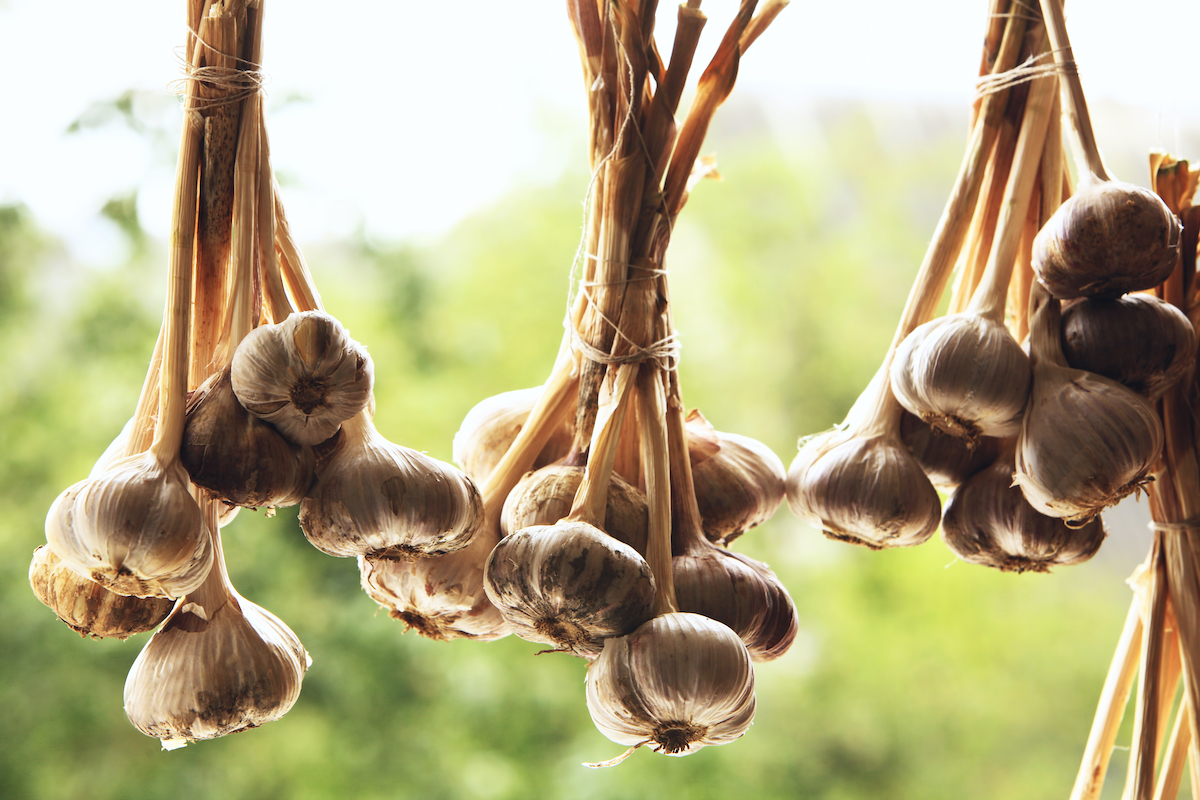
\includegraphics[width=.8\linewidth]{optique/optiquegeometrique/ail.jpg}
    \caption{Photographie d'une gousse d'ail.}
\end{figure}


\paragraph{Résolution de problème :}
\begin{questions}
    \question En vous aidant de la photographie fournie, déterminer la taille des gousses d’ail sur la pellicule. En déduire $d$ et $D$.
    \question On voit sur la photos des ronds clairs qui viennent d’objets au loin. Déterminer leur taille sur la pellicule, en déduire le rayon
du diaphragme $R$. Donner le nombre d'ouverture de l'appareil $\frac{f'}{2R}$.
    \question À quel phénomène aurait-on pu penser pour expliquer ronds ? Montrer quantitativement que ce n’est pas dû à cette cause.
    \question Quelle semble être la distance maximale jusqu’à laquelle on voit net ? En déduire la taille d’un élément photosensible sur cette
pellicule. Comparer à la résolution en pixels d’un appareil récent.
\end{questions}

\end{exercise}

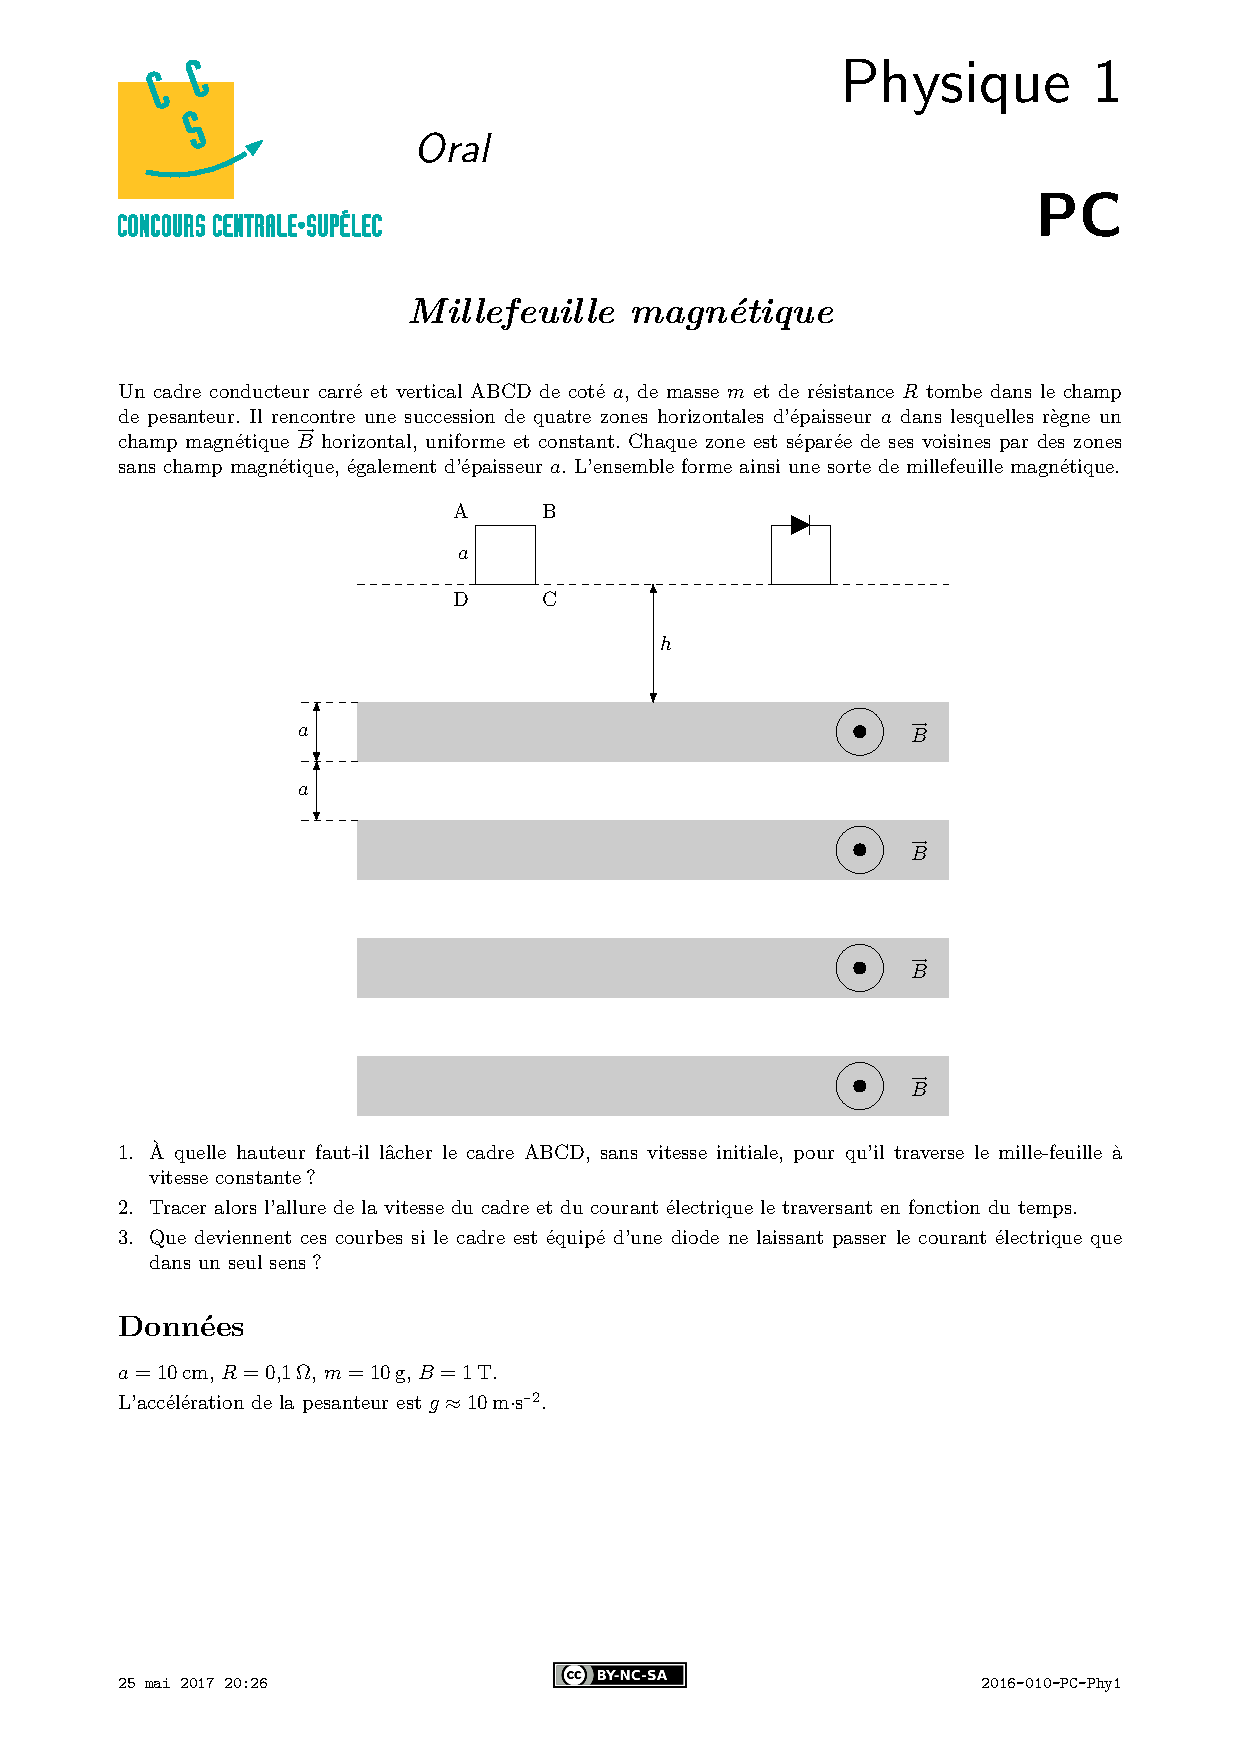
\includepdf[pages=-]{oraux/centrale/Centrale2016.pdf}

%
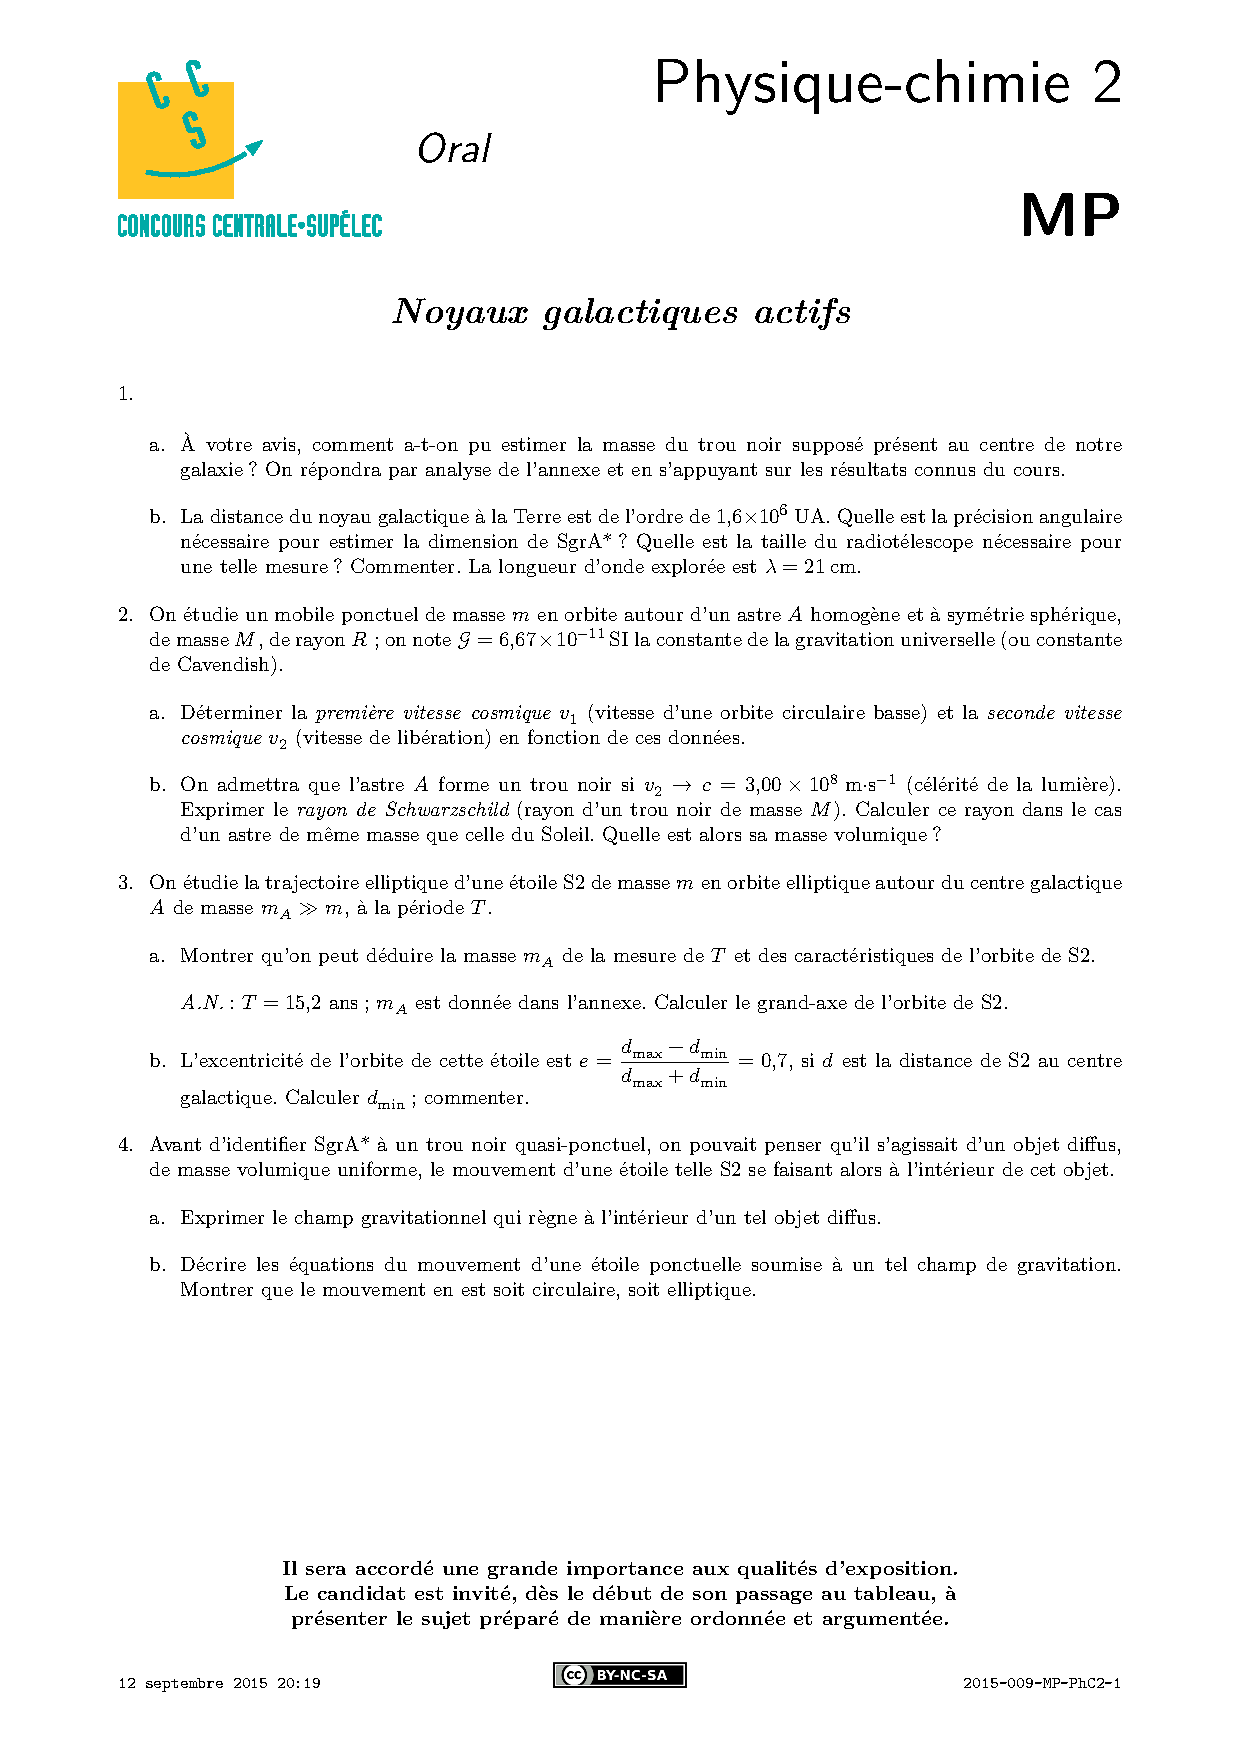
\includepdf[pages=-]{oraux/centrale/Centrale2015.pdf}


\begin{exercise}{Précession du périhélie de Mercure}{-1}{Spé}
{meca}{centrale}

Le but de cet exercice est d'appliquer une correction post-newtonienne venant de la théorie de la relativité générale à la trajectoire de Mercure afin d'expliquer l'anomalie de la précession de la périhélie de Mercure dont une partie n'est pas expliquée par la mécanique newtonienne.

\paragraph{Résolution de problème :}~

On considère le Soleil fixé au point $O$, on notera $M$ l'emplacement de Mercure, $\vec{r} = \vec{OM}$ et $\vec{v} = \dv{\vec{r}}{t}$.

À $t = 0$, on suppose Mercure à sa périhélie, et on fixe l'origine des angles de manière à ce que $\theta = 0$ à $t=0$.

\begin{questions}
    \question En calculant la valeur du vecteur $\vec{h} = \vec{r} \cross \vec{v}$, montrer que la trajectoire de Mercure est située dans un plan contenant le Soleil et qu'elle obéit à la deuxième loi de Kepler.
    \question Quelle est la forme de la trajectoire décrite par Mercure autour du Soleil ? En utilisant les documents en annexe, donner la valeur numérique du demi-grand axe et de l'excentricité de cette trajectoire.
    \uplevel{On introduit le vecteur de Laplace $\vec{A} = \alpha \frac{\vec{r}}r + \vec{v} \cross \vec{h}$.}
    \question Montrer que pour une valeur bien choisie de $\alpha$ on a $\dv{\vec{A}}{t} = \vec{0}$. \\ On gardera cette valeur pour la suite.
    \question Calculer la norme de $\vec{A}$ en fonction de $\alpha$, $h$ et la distance Mercure-Soleil à la périhélie et montrer que le vecteur $\vec{A}$ pointe toujours vers la périhélie de Mercure.
    
    \question Montrer, en calculant $\vec{A}\cdot\vec{r}$ de deux manières différentes, l'égalité $\alpha + \frac{h^2}{r} = \norm*{\vec{A}}\cos(\theta)$.\\ En déduire $r(\theta)$. Montrer, en s'appuyant sur les documents, que la trajectoire est bien une ellipse.
    \uplevel{On souhaite retrouver la valeur de la précession (l'angle $\Delta \phi$ dont a tourné l'orbite en une révolution) de Mercure. Pour cela, on introduit une force fictive s'appliquant à Mercure en plus de l'attraction du Soleil, qui vaut $$\vec{F}_\textsc{PN}=-\gamma \frac{G m M_\odot a}{r^3}\frac{\vec{r}}{r},$$
    où $a$ est le demi-grand axe de l'orbite de Mercure, $G$ la constante gravitationnelle et $M_\odot$ la masse du Soleil.}
    \question Quelle est l'unité de $\gamma$ ? On donne $$\gamma = \frac{6 G M_\odot}{c^2a}.$$
    Estimer numériquement sa valeur. Peut on considérer $\gamma \ll 1$ ?
    \question Les résultats de la première question sont-ils toujours valables ?
    \question Calculer la nouvelle valeur de $\dv{\vec{A}}{t}$. Le vecteur $\vec{A}$ est-il toujours constant ?
    \uplevel{On définit le vecteur
    $\displaystyle \vec{u} = \frac{\vec{h} \cross \vec{A}}{hA}$
    , avec $h$ et $A$ les normes de $\vec{h}$ et $\vec{A}$, respectivement.}
    \question Quelle est la direction de $\vec{u}$ ? Sa norme ?
    \question Calculer la quantité $$\dv{\phi}{t}(\theta) = \vec{u}\vdot \dv{\vec{A}}{t}\frac{1}{A}.$$
    Que représente cette quantité ?
    \question La précession $\Delta \phi$ est donnée par la formule 
    $$\Delta \phi = \int_{(T)} \dv{\phi}{t}\dd{t} = \int_0^{2\pi}\dv{\phi}{t}\dv{t}{\theta}\dd{\theta}$$
    Interpréter cette formule et calculer la valeur de $\Delta \phi$. Est-ce cohérent avec la formule donnée en annexe ?
    \question Faire l'application numérique. La correction post-newtonienne permet-elle d'expliquer l'anomalie de la périhélie de Mercure ?
\end{questions}

\end{exercise}
\pagebreak

\printexerciseheader

\begin{center}
    \itshape --- \quad \textbf{Annexe (page 1)} \quad ---
\end{center}

\paragraph{Document 1 :}\textsf{Mercure}
\begin{center}\begin{minipage}{.9\textwidth}
Mercure est la planète la plus proche du Soleil et la moins massive du Système solaire. Son éloignement au Soleil est compris entre 0,31 et 0,47 unité astronomique (soit 46 et 70 millions de kilomètres), ce qui correspond à une excentricité orbitale de 0,2 — plus de douze fois supérieure à celle de la Terre, et de loin la plus élevée pour une planète du Système solaire. Elle est visible à l'œil nu depuis la Terre avec un diamètre apparent de 4,5 à 13 secondes d'arc. 

[...]

Comme pour l'ensemble des planètes du Système solaire, l'orbite de Mercure connaît une très lente précession du périhélie autour du Soleil, c'est-à-dire que son orbite est elle-même en rotation autour du Soleil. Cependant, contrairement aux autres planètes, la période de précession du périhélie de Mercure ne concorde pas avec les prédictions faites à l'aide de la mécanique newtonienne.

En effet, Mercure connaît une précession légèrement plus rapide que celle à laquelle on peut s'attendre en appliquant les lois de la mécanique céleste, et se trouve en avance d'environ 43 secondes d'arc par siècle. 

[...]

En 1916, Albert Einstein avance la théorie de la relativité générale. En appliquant les paramètres dits post-képlériens de sa théorie au mouvement de Mercure, Einstein fournit l'explication de la précession observée en formalisant la gravitation comme étant affectée par la courbure de l'espace-temps. La formule de précession subie par l'orbite en une période obtenue par Einstein est :

\begin{align*}
    \Delta \phi_{\text{Einstein}} = \frac{6\pi G M_\odot}{c^2 a (1-e^2)}
\end{align*}

où $a$ est le demi-grand axe de l'ellipse, $e$ son excentricité, $G$ la constante gravitationnelle, $M_\odot$ la masse du Soleil, et $c$ la vitesse de la lumière dans le vide.
\end{minipage}\end{center}
\textsl{Extrait adapté de Wikipédia, l'encyclopédie libre.}

\paragraph{Document 2 :}\textsf{La précession du périastre}
\begin{center}\begin{minipage}{.9\textwidth}
En astronomie, la précession du périastre est le phénomène selon lequel un corps en orbite autour d'un autre (par exemple une planète autour d'une étoile) voit l'ellipse décrivant sa trajectoire tourner lentement dans le plan orbital de l'objet. Cela se traduit par le fait qu'au cours des révolutions successives de l'objet, la direction décrite par la droite passant par le corps central et le corps en orbite au moment où ils sont les plus proches (le périastre) n'est pas fixe, mais varie lentement.
\end{minipage}\end{center}
\begin{figure}[H]
    \centering
    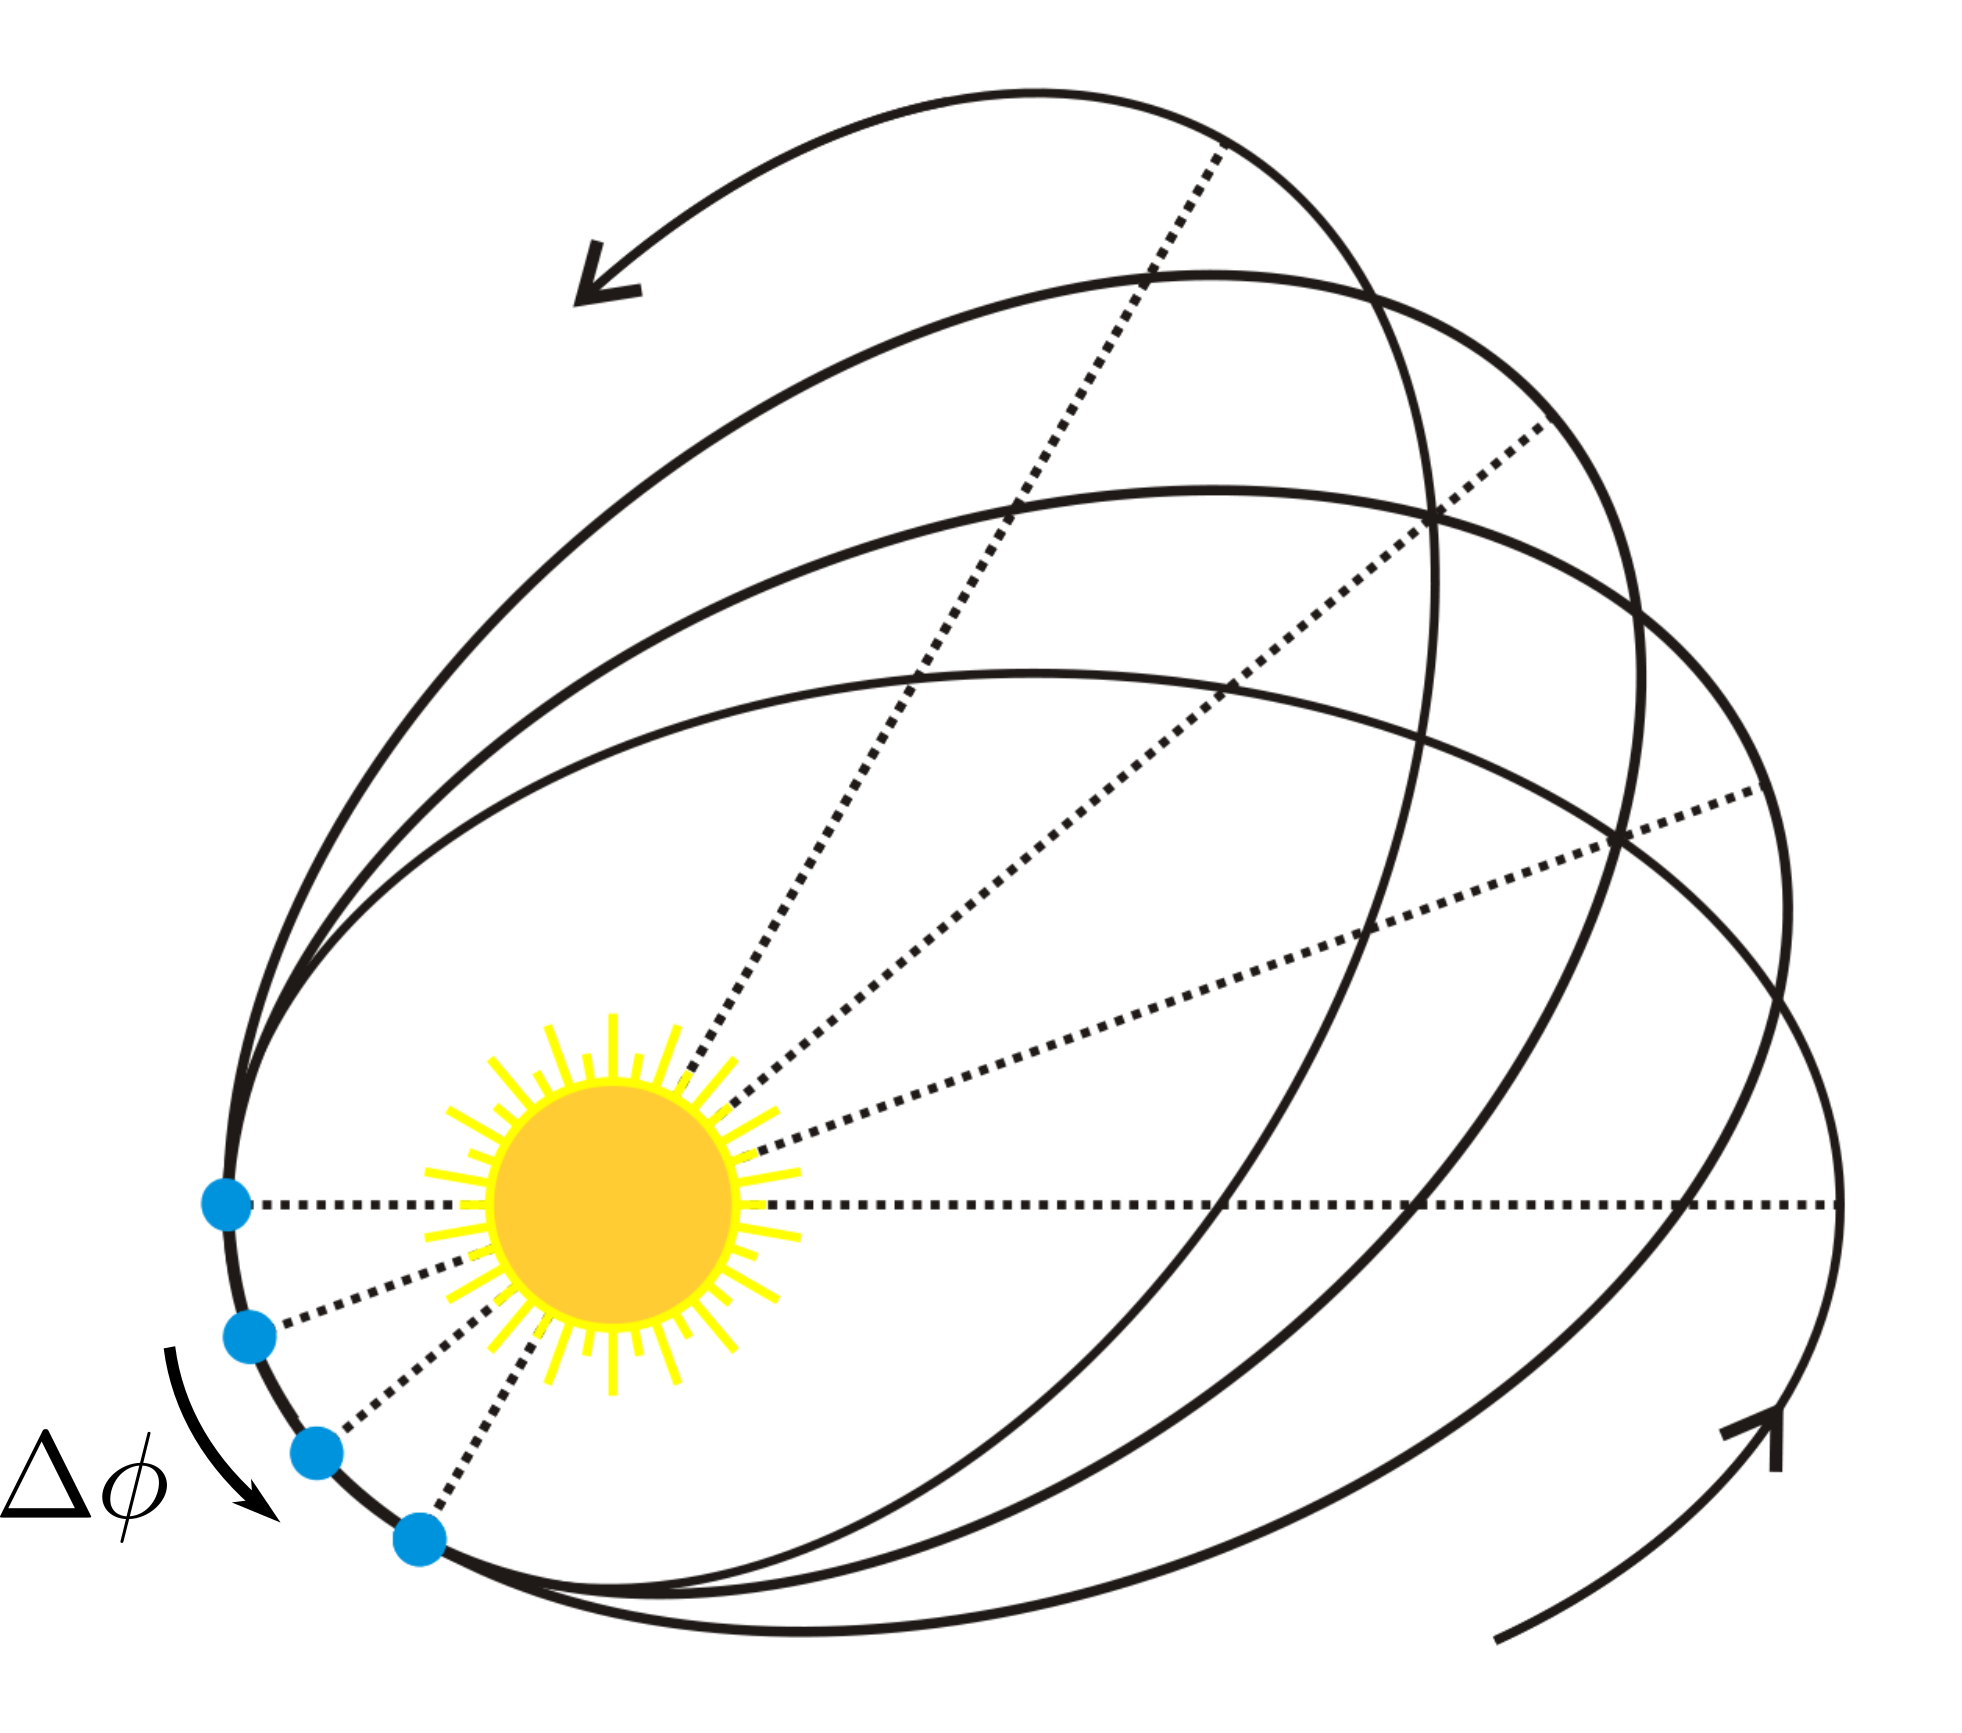
\includegraphics[width=0.3\linewidth]{oraux/centrale/perihelion_precession_dphi.png}
\end{figure}
\begin{center}\begin{minipage}{.9\textwidth}
Précession de périastre (très exagérée) : Le périastre (en bleu) tourne lentement autour de l'astre. À chaque orbite effectuée par l'objet, le périastre de déplace d'un angle $\Delta \phi$.  
\end{minipage}\end{center}
\pagebreak

\printexerciseheader

\begin{center}
    \itshape --- \quad \textbf{Annexe (page 2)} \quad ---
\end{center}

\paragraph{Document 3 :}\textsf{L'ellipse en mécanique céleste}
\begin{center}\begin{minipage}{.9\textwidth}
En mécanique képlerienne, les trajectoires des planètes sont des ellipses, dont l'un des foyers est l'astre autour duquel elles orbitent.

Pour paramétriser une ellipse dont on connaît le foyer et l'orientation du périastre, il suffit de connaître deux des grandeurs caractéristiques de l'ellipse, les autres pouvant s'en déduire facilement.

Traditionnellement, on paramétrise les ellipses en mécanique du ciel par deux grandeurs : le \textbf{demi-grand axe}, noté $a$, et l'\textbf{excentricité}, notée $e$. Le demi-grand axe est une longueur représentant l'extension spatiale de l'ellipse, tandis que l'excentricité est un nombre sans dimension compris entre 0 et 1 qui représente l'écart entre l'ellipse et un cercle (une ellipse d'excentricité 0 étant un cercle).

L'équation polaire d'une ellipse si on prend comme centre l'un des foyers est 
$$ r(\theta) = \frac{p}{1+e\cos(\theta)} $$
Où $p = a(1 - e^2)$ est appelé le \textbf{paramètre} de l'ellipse.
\end{minipage}\end{center}
\begin{figure}[H]
    \centering
    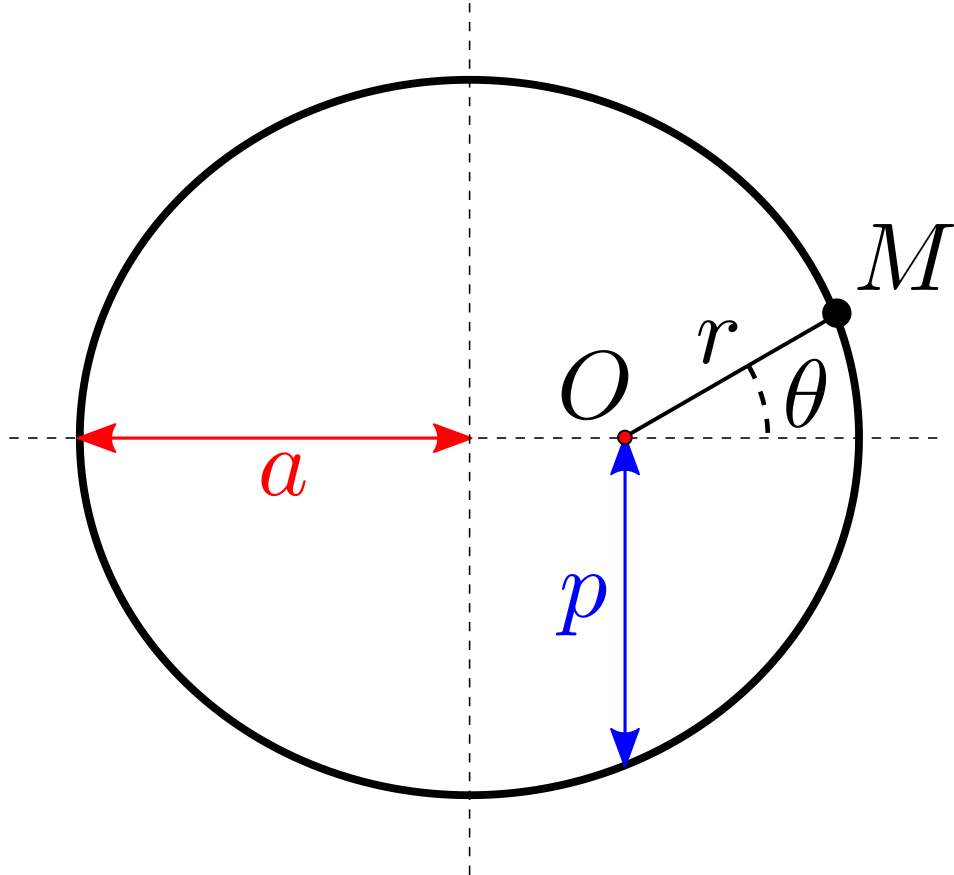
\includegraphics[width=0.4\linewidth]{oraux/centrale/EllipseVal_big.png}
\end{figure}
\begin{center}\begin{minipage}{.9\textwidth}
Paramétrisation d'une ellipse : Pour une ellipse quelconque, sont représentés le demi-grand axe $a$ et le paramètre $p$.
\end{minipage}\end{center}

\paragraph{Document 4 :}\textsf{La seconde d'arc}
\begin{center}\begin{minipage}{.9\textwidth}
La seconde d'arc correspond à une unité de mesure d'un angle. Son symbole est '', mais on peut également la noter arcsec. On l'emploie pour mesurer de très petits angles. Lorsque plus de précision est nécessaire, il est possible d'utiliser, devant l'expression seconde d'arc, les mêmes préfixes que pour les unités SI. Ainsi il existe des millisecondes d'arc, microsecondes d'arc ou encore des nanosecondes d'arc.

La seconde d'arc est définie par rapport au degré. En géométrie, on peut en effet diviser le cercle en 360 parties égales que l'on nomme degré ($ ^{\circ}$). Lorsque la mesure doit se montrer plus précise, il faut faire appel aux sous-unités du degré. La première d'entre elles est la minute d'arc ('). Comme une heure se divise en 60 minutes, un degré se divise en 60 minutes d'arc. Et comme une minute se divise en 60 secondes, une minute d'arc se divise aussi en 60 secondes d'arc. Ainsi entre le degré et la seconde d'arc, il existe un facteur 3 600, comme entre l'heure et la seconde.
\end{minipage}\end{center}
\textsl{D'après \texttt{www.futura-sciences.com}}


\paragraph{Document 5 :}\textsf{Données numériques}
\begin{itemize}
    \item Constante gravitationnelle : $6.674 \times 10^{-11}$ S.I.
    \item Masse du Soleil : $1,989 \times 10^{30}$ kg
\end{itemize}

\newpage
\begin{exercise}{Tube fluorescent}{-1}{Spé}
{\'Electrocinétique}{centrale}

Un tube fluorescent est une lampe électrique de forme tubulaire, de la famille des lampes à décharge à basse pression. Il contient du mercure à l'état gazeux, dont les atomes sont ionisés sous l'effet d'un courant électrique appliqué entre les électrodes placées à chaque extrémité du tube ; ils émettent alors par luminescence un rayonnement essentiellement ultraviolet, qui est converti en lumière visible par la poudre fluorescente déposée sur les parois du tube. La couleur de la lumière émise dépend de la nature de la poudre fluorescente utilisée.

Le tube fluorescent est souvent désigné à tort par l'expression tube au néon, alors que le tube néon est un autre type de lampe à décharge, de couleur rouge, qui n'utilise pas la fluorescence.

Un tube fluorescent peut se comporter de deux façons :
\begin{itemize}
    \item Éteint : Lorsque le tube est éteint, il n'émet pas de lumière et il se comporte électriquement comme un interrupteur ouvert et le courant ne peut pas passer.
    \item Allumé : Lorsque le tube est allumé, il émet de la lumière et il se comporte électriquement comme une résistance de valeur $R_t$.
\end{itemize}
Un tube fluorescent s'allume quand la tension à ses bornes dépasse une certaine tension d'allumage $U_a$. Un fois allumé, le tube ne s'éteint que lorsque la tension descend en dessous de $U_e$, la tension d'extinction.

\paragraph{Résolution de problème :}~\\
Le but de la démarche est de déterminer les caractéristiques d'un tube fluorescent inconnu.

On adopte le montage suivant: Un générateur de tension de f.e.m. $E = 100$~V associé à une résistance $R$ alimente un tube fluorescent $T$. Un condensateur de capacité $C = 2200$~$\mu$F est branché en parallèle du tube.

\begin{circuit}[Schéma du montage utilisé.]

      \draw (0,0)
      to [vsource, v^>=$E$] (0,1.5)
      to [R, l=$R$] (0,3)
      to [short] (2, 3)
      to [short, *-*] (2,0)
      to [short] (0,0) node [ground] at (0,0) {};
      
      \draw (2,3) to [short] (4,3)
      to [C, l^=$C$] (4,0)
      to [short] (2,0) {};
      % \draw (5.3,0) [open, v_=Voltmètre] to (5.3,3) {} ;
      % \draw [red, dashed] (1.4,-0.2) rectangle(2.6,3.2) ;
      % \node [red] at (2.0,3.5) {Tube fluorescent};

      \filldraw[fill=white](2, 1.5) circle(0.4);
      \node [black] at (2.0,1.5) {$T$};
\end{circuit}

À $t<0$, le condensateur est déchargé et le tube est éteint. On allume le générateur à $t=0$.

Pour faire des mesures, on ne dispose que d'un chronomètre et d'un voltmètre branché aux bornes du tube.

On réalise deux expériences en utilisant deux résistances $R$ différentes
\begin{itemize}
    \item Lors de la première expérience ($R = 5$~$\Omega$) le tube s'allume presque immédiatement. Il reste allumé et très rapidement le tension à ses bornes se stabilise à 90 $V$.
    \item Lors de la seconde expérience ($R = 500$~$\Omega$) le tube s'allume à $t=1.8$~s, puis oscille de manière régulière entre l'état éteint et allumé. La durée de 10 cycles est de 7.6~s.
\end{itemize}


\begin{questions}
    \question Reproduire le circuit équivalent dans le cas où le tube est allumé et dans le cas où il est éteint. 
    
    \question Montrer qu'il existe différents régimes possibles en fonction des valeurs du paramètre sans dimensions $\displaystyle k = \frac{R_t}{R+R_t}$. Expliquer qualitativement les phénomènes observés.
    
    \question Déterminer les valeurs $U_a$, $U_e$ et $R_t$ pour le tube utilisé.
\end{questions}



% \paragraph{Données :} $E = 100$ V, $R_g = 500$ $\Omega$, $C = 2000$ $\mu$F, $U_a$ = 80 V, $U_e$ = 40 V

\end{exercise}

\begin{solution}

À chaque fois on utilise la loi du condensateur + la loi des mailles. Pour le tube allumé, on peut passer par la représentation de thévenin équivalente si on est rapide.
\begin{itemize}
    \item \textbf{TUBE ETEINT :} On a $RC \dot{u} + u = E$, la tension tend vers $E$ avec un temps caractéristique $\tau = RC$
    \item \textbf{TUBE ALLUME :} On a $kRC \dot{u} + u = kE$, la tension tend vers $kE < E$ avec un temps caractéristique $\tau = kRC < RC$
\end{itemize}

\textbf{Explications des observations: }

Dans la premières expérience le tube reste allumé, donc $kE > U_e$. 

Dans la seconde expérience, le tube s'éteint donc $kE < U_e$. Une fois éteint la tension monte à nouveau, le tube s'allume etc, d'où les oscillations.

\textbf{Détermination de $R_t$: } D'après l'expérience 1, on a $k_1E = 90$~V, d'où l'on déduit $R_t = R_1\frac{u_\infty}{E-u_\infty} = 45$~$\Omega$.

\textbf{Détermination de $U_a$: } Le temps d'allumage $t_{all}$ est tel que $U_a = E(1-e^{-t/RC})$. Dans l'expérience 1 on a $RC = 11$~ms donc on n'a le temps de rien voir. Dans l'expérience 2, $RC = 1.1$~s, d'où $U_a = 80$~V

\textbf{Détermination de $U_e$: } Il faut utiliser l'expérience 2. On a $k_2 \approx 0.08 \ll 1$ donc en première approximation le temps d'oscillation est le temps de montée (le tube est le plus souvent éteint). On a alors la condition $U_a = U_e + (E-U_e)(1-e^{-T/RC})$. On en déduit 
$$
U_e = \frac{U_a - E (1-e^{-T/RC})}{e^{-T/RC}}
$$
ici $e^{-T/RC} \approx 0.5$ d'où $U_e = 60$~V

\end{solution}
\begin{exercise}{Portrait de phase OHA}{-1}{Spé}
{Méca, Référentiel non galiléen}{centrale}

On considère le référentiel du laboratoire est supposé galiléen. Une boule de masse $m$ de rayon $R$ est reliée à un point fixe $O$ par une tige rigide de longueur $\ell$, de masse négligeable par rapport à $m$, et de dimensions latérales négligeables. La boule est libre de tourner autour de l'axe $Oz$ de telle sorte que sa trajectoire est comprise dans le plan $Oxy$. On considèrera également l'accélération de la pesanteur dirigée suivant $-\ve_y$.

Ce dispositif baigne dans un fluide en rotation solide autour de l'axe $Oz$ avec une vitesse angulaire constante $\Omega$. On note $\gamma$ le coefficient de frottement du fluide et $\rho$ sa masse volumique. On suppose la densité de la boule supérieure, \underline{mais relativement proche} de celle du fluide. Le fluide exerce sur la boule une force de frottement visqueux
$$\vec{F} = -m\gamma\vv_\text{r},$$
où $\vv_\text{r}$ est la vitesse relative de la boule par rapport au fluide.

\begin{center}
    \begin{tikzpicture}
    
    \draw[->, black!30] (-2, 0) -- (3, 0);
    \draw (3,0) node[below=2pt] {$x$};
    
    \draw[->, black!30] (0, -2) -- (0, 3);
    \draw (0,3) node[right=2pt] {$y$};
    
    
    \draw (0, 0) circle (0.15cm) node [below left=2pt, thick, black] {$z$};
    \filldraw [black] (0,0) circle (0.05cm);
    
    \coordinate (O) at (0, 0);
    \draw (O) node[above left=2pt] {$O$};
    
    \coordinate (m) at (1.5, -1.5);
    \fill[black] (m) circle (0.15);
    \draw (m) node[below right=2pt] {$R, m$};
    
    \draw[thick] (O) -- (m);
    \path (O) -- node [midway, above right=1pt] {$\ell$} (m);
    
    \newcommand\RT{1.5}
    \draw[->] (0, -\RT) arc(-90:-45:\RT);
    \draw (0.38*\RT, -0.92*\RT) node[below=2pt] {$\theta$};
    
    
    \newcommand\RO{3}
    \draw[->, thick] (-0.94*\RO,0.34*\RO) arc(160:200:\RO);
    \draw (-\RO, 0) node[left=2pt] {$\Omega$};

    
    \draw[->, thick] (2, 1.5) -- (2, 0.5);
    \draw (2,1) node[right=2pt] {$\vec{g}$};
    
    
    
    \end{tikzpicture}
\end{center}


\paragraph{Exercice :}
\begin{questions}
    \question Montrez que $\theta(t)$ vérifie l'équation différentielle suivante
    \begin{equation}
        \dfrac{1}{\tau}\ddot{\theta} + \dot{\theta} + \alpha\sin\theta = \Omega,
    \end{equation}
    avec $\tau$ et $\alpha$ des paramètres dont vous donnerez l'expression. Interprétez cette équation.
    
    \question En comparant des échelles de temps que vous introduirez, donner les conditions pour négliger
    \begin{parts}
        \part l'accélération de la boule ;
        \part les frottements ;
        \part la gravité ;
        \part la rotation solide du fluide.
    \end{parts}
    
    \question Déterminez les éventuelles positions d'équilibre du système ; précisez les conditions d'existence de telles positions. Étudiez (par la méthode de votre choix) leur stabilité.
    
    \uplevel{Vous disposez d'un programme écrit en langage \texttt{python} qui permet de résoudre numériquement l'équation différentielle et de tracer la solution $\theta(t)$.}
    
    \question Tracer la trajectoire du système. Modifier le code pour tracer également le portrait de phase du système ($\dot{\theta}$ vs $\theta$) et vérifier la cohérence des résultats précédents.
    
    \uplevel{On se place désormais dans la situation 2.1 ou l'accélération de la boule est négligeable. \\
    On prendra $\tau = 10^{-2}$ et $\alpha = 1$ dans le code.}
    
    \question Réécrire l'équation de la dynamique de la boule sous la forme
    \begin{equation}
        \dot{\theta} + \alpha\sin\theta = \Omega.
    \end{equation}
    
    \question En fonction des cas que vous avez établis à la question 3, donner le temps de retour à l'équilibre ou la période du système par un calcul. Vérifier la cohérence ensuite avec le programme python.
    
\end{questions}

\paragraph{Données :}~\\
$$\int_0^{2\pi} \dfrac{\dd{u}}{1 - x \sin u} \sim^{x \rightarrow 1^-} \dfrac{\pi\sqrt{2}}{\sqrt{1-x}}.$$

\end{exercise}


\section{Mines Ponts}
\begin{exercise}{Particule autour d'un fil}{-1}{Spé}
{}{mines}

\paragraph{Question de cours} \textsf{(15 minutes préparation, 10 minutes de passage) \textbf{:}}

Machines thermiques dithermes.

\paragraph{Exercice} \textsf{(15 minutes préparation, 15 minutes de passage) \textbf{:}}

On considère un fil conducteur infini parcouru par un courant $I$ constant. 

\begin{questions}
\question On place à une distance $a$, de part et d'autre symétriquement par rapport à ce fil deux particules de charge $q$, initialement immobiles. Trouver les équations régissant ce problème. Montrer qu'il est possible de se ramener à une équation différentielle ordinaire suivant la coordonnée $r$ uniquement.

\question On place cette fois-ci à une distance $a$ du fil une seule particule de charge $q$ possédant une vitesse initiale $\vec{v_0}=v_0\ve_r$. Quels sont les changements par rapport à la situation précédente ?
\end{questions}


\paragraph{Données :}~\\
\begin{align*}
    \int_{1/e}^{e} \frac{\dd{x}}{\sqrt{1-\ln(x)^2}} \approx 3.98
\end{align*}

\end{exercise}

\begin{exercise}{Bilan entropique}{-1}{Spé}
{}{mines}

\paragraph{Question de cours} \textsf{(15 minutes préparation, 10 minutes de passage) \textbf{:}}

Mouvements dans un champ de force centrale conservatif. Énergie potentielle effective.

\paragraph{Exercice} \textsf{(15 minutes préparation, 15 minutes de passage) \textbf{:}}

On considère une tige de masse volumique $\rho$, de section $\Sigma$ et de longueur $L$. La température de chacune de ses extrémités est maintenue constante par des thermostats à la température $T_1$ (en $x=0$) et $T_2$ (en $x=L$). La tige est calorifugée sur les côtés.

\begin{questions}
\question On se place dans le régime stationnaire. Quel est le profil de température stationnaire $T(x)$ ?

\question Déterminer l'entropie créée par unité de temps pour une tranche de longueur $\dd{x}$, puis pour toute la tige.

\question On retire les thermostats et on isole la barre de sorte à ce qu'elle n'échange plus de chaleur avec l'extérieur. Après un certain temps, que devient le profil de température ? Calculer la variation d'entropie de la tige.
\end{questions}

\end{exercise}

\begin{exercise}{Les délires d'un complotiste}{-1}{Spé}
{}{mines}

\paragraph{Question de cours} \textsf{(15 minutes préparation, 10 minutes de passage) \textbf{:}}

Trous d'Young et dualité onde--corpuscule.

\paragraph{Résolution de problème} \textsf{(15 minutes préparation, 15 minutes de passage) \textbf{:}}

M. Laforce, complotiste anti-vaccin, veut se protéger des ondes de la 5G dont il a très peur à l'aide d'une simple feuille d'aluminium.

En enroulant un téléphone portable dans la feuille d'aluminium, peut-on encore recevoir des appels ?

Vous répondrez à la question en calculant la puissance transmise par le téléphone à travers la feuille d'aluminium.

\paragraph{Données :}
\begin{itemize}
    \item Permittivité du vide $\mu_0 = 4\pi\times 10^{-7}$ H$\cdot$m$^{-1}$ ;
    \item Vitesse du son dans le vide $c = 3,0 \times 10^8$ m$\cdot$s$^{-1}$ ;
    \item Masse volumique de l'aluminium $\rho_\text{Al} = 2,7$ g$\cdot$cm$^{-3}$ ;
    \item Conductivité de l'aluminium $\sigma = 2\times 10^7$ S$\cdot$m$^{-1}$ ;
    \item Numéro atomique et nombre de masse de l'aluminium $Z = 13$, $A = 27$ ;
    \item Un rouleau d'aluminium de 30 mètres acheté dans le commerce a un rayon intérieur de 2 cm et un rayon extérieur de 2,5 cm
    \item Bande de fréquences de la 5G : 3,5---3,8 GHz 
\end{itemize}

\end{exercise}

\begin{exercise}{Tube tournant}{-1}{Spé}
{}{mines}

\paragraph{Question de cours} \textsf{(15 minutes préparation, 10 minutes de passage) \textbf{:}}

Équations de Maxwell, forme locale et intégrale.

\paragraph{Exercice} \textsf{(15 minutes préparation, 15 minutes de passage) \textbf{:}}

On considère un tube de section circulaire formant un demi cercle de rayon $R$. Une bille de masse $m$ est placée dans ce tube et peut s'y mouvoir sans frottement. Le tube est mis en rotation autour de son axe de symétrie vertical à la pulsation $\omega$.


\begin{center}
    \begin{tikzpicture}
    
    \draw[->, black!30] (0, -1) -- (0, 3);
    \draw (0,3) node[right=2pt] {$z$};
    
    \draw (-2.5,2) arc(-180:0:2.5);
    \draw (-2.2,2) arc(-180:0:2.2);
    
    \fill[black] (0.5*2.35,2-0.866*2.35) circle (0.15);
    \draw (0.5*2.35,2-0.866*2.35) node[below right=2pt] {$m$};
    
    \draw [xshift=0.3cm,rotate around={180:(-0.4,2.2)},line width=1pt,-stealth] (-0.25,2) arc (-30:210:0.3cm and 0.2cm) node[below right=0.1cm] {$\omega$};
    
    \draw[->, thick] (4, 1.5) -- (4, 0.5);
    \draw (4,1) node[right=2pt] {$\vec{g}$};
    
    \end{tikzpicture}
\end{center}

\begin{questions}
\question Trouver la (ou les) position(s) d'équilibre de la bille en fonction des paramètres du problème.

\question En partant d'une position d'équilibre, quelle quantité minimale d'énergie faut-il fournir à la bille pour qu'elle soit éjectée du tube ?

\question Que se passe-t-il si l'on incline le dispositif par rapport à la verticale ?
\end{questions}

\end{exercise}

\begin{exercise}{Effet Ramsauer-Townsend}{-1}{Spé}
{}{mines}

\paragraph{Question de cours} \textsf{(15 minutes préparation, 10 minutes de passage) \textbf{:}}

Transfert de chaleur conductif : Principe et applications.

\paragraph{Exercice} \textsf{(15 minutes préparation, 15 minutes de passage) \textbf{:}}

On considère une particule quantique de masse $m$ et d'énergie $E > 0$ provenant de $-\infty$ et  se déplaçant dans le sens de $x$ croissants, arrivant sur un puits de potentiel de largeur $a$ et de profondeur $V_0$.


\begin{center}
    \begin{tikzpicture}
    
    % \draw (0,0) node[below=2pt] {$0$};
    \draw[->, black!30] (-5, 0) -- (5, 0);
    \draw (5,0) node[below=2pt] {$x$};
    % \draw[->, black!30] (0, 0) -- (0, 3);
    % \draw (0,3) node[right=2pt] {$V(x)$};
    
    \draw[thick, dashed] (-5, 0.5) -- (5, 0.5);
    \draw (5,0.5) node[above=2pt] {$E$};
    
    \draw[thick] (-5,  0) -- (-1,  0);
    \draw[thick] (-1,  0) -- (-1, -1);
    \draw[thick] (-1, -1) -- ( 1, -1);
    \draw[thick] (1 , -1) -- ( 1,  0);
    \draw[thick] (1 ,  0) -- ( 5,  0);
    
    \draw[<->] (-1, -1.2) -- (1, -1.2);
    \draw (0,-1.2) node[below=2pt] {$a$};
    
    \draw (1,-1) node[right=2pt] {$-V_0$};
    
    \end{tikzpicture}
\end{center}

\begin{questions}
\question Justifier l'existence d'une probabilité de réflexion de la particule. Comparer à la situation correspondante en mécanique classique.

\question Exprimer le coefficient de réflexion $R$ du puits en fonction de $a$, $E$, $V_0$. Pour quelles énergies a-t-on une résonance en réflexion ?
\end{questions}


\end{exercise}

\begin{exercise}{Ressort et physique statistique}{-1}{Spé}
{}{mines}

\paragraph{Question de cours} \textsf{(15 minutes préparation, 10 minutes de passage) \textbf{:}}

Filtrage linéaire en électronique.

\paragraph{Exercice} \textsf{(15 minutes préparation, 15 minutes de passage) \textbf{:}}

On considère une particule de masse $M$ attachée à un ressort, de raideur $k$ et de longeur à vide $\ell$. Elle subit les frottements visqueux de l'air avec un coefficient $\alpha$. On négligera tout frottement solide et action de la gravité.

On lui applique un forçage sinusoïdal d'amplitude $F_0$ et de pulsation $\omega$.

\begin{questions}
    \question Donner l'amplitude des oscillations de la particule. Dans quelles conditions observe-t-on une résonance ? Quelle est alors la pulsation de résonance $\omega_0$ ? Quel est le temps typique du régime transittoire $\tau$ ?
    \uplevel{On suppose maintenant que de petites particules de masse $m$ se déposent sur la grande particule.}
    \question Déterminer une expression approchée (de la forme $\omega_0 - \delta\omega$) de la nouvelle pulsation de résonance quand $n$ petites particules se déposent sur la grande. Quel est l'intérêt d'un tel dispositif ?
    \uplevel{On considère que la grande particule possède $N$ sites où de petites particules peuvent se déposer. On suppose également que l'énergie d'adhésion d'une petite particule est $\varepsilon$.}
    \question Donner la probabilité qu'un site soit occupé. En déduire le nombre moyen de sites occupés, ainsi qu'un ordre de grandeur des fluctuations du nombre de sites occupés autour de cette moyenne.
    \question En déduire une estimée de la pulsation de résonance du système.

\end{questions}

\end{exercise}

\begin{exercise}{Dynamo}{-1}{Spé}
{}{mines}

\paragraph{Question de cours}~

Mesure d'une enthalpie standard de réaction par calorimétrie.

\paragraph{Exercice}~

On considère le dispositif suivant composé d'un cylindre conducteur en rotation à la vitesse angulaire $\Omega$  et soumis à un frottement visqueux $\alpha$ (en haut), relié à un système de spires de résistance totale $R$ et d'inductance $L$ parcourues par un courant $I$ générant un champ magnétique $\vec{B}$ supposé uniforme au niveau du disque (en bas).

\begin{center}
    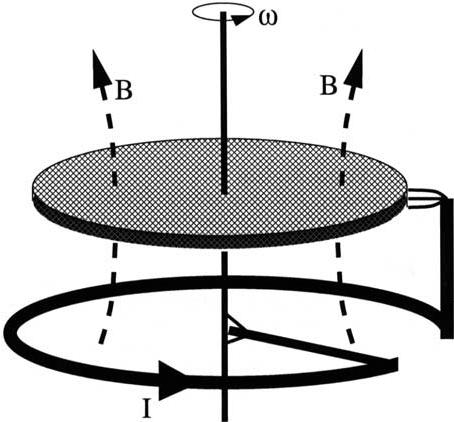
\includegraphics[width=.5\linewidth]{oraux/mines/bullard-dynamo.png}
\end{center}

On considère tout d'abord que le courant $I$ du système est constant.

\begin{questions}
\question Exprimer le lien entre le champ $B$ au niveau de la spire et le courant $I$.
\question Justifier l'existence d'une force de Laplace au niveau du cylindre. En déduire l'équation de la dynamique du système et montrer que la vitesse de rotation $\Omega$ du système croît jusqu'à une valeur limite en un temps $\tau$ qu'on précisera tous deux.
\uplevel{On fixe maintenant la vitesse de rotation $\Omega$, mais le courant $I$ n'est plus constant.}
\question En notant $e$ la force électromotrice induite dans le circuit, établir l'équation de la dynamique électrique du circuit.
\question Par un argument énergétique, déterminer la valeur de $e$.
\question Montrer que au dessus d'une vitesse de rotation seuil $\Omega_c$, le courant dans le système croit exponentiellement. En quoi cela est surprenant ?
\end{questions}

% \begin{questions}
% \question Donner l'expression de la force de Laplace exercée par le champ magnétique sur le cylindre. Quel est son effet d'un point de vue dynamique ?
% \question En déduire l'équation de la dynamique mécanique du système et montrer que la vitesse de rotation $\Omega$ du système croit jusqu'à une valeur limite en un temps $\tau$ qu'on précisera tout deux.
% \uplevel{Le champ magnétique $B$ et le courant $I$ ne sont toutefois pas constants.}
% \question Décrire qualitativement ce qu'il se passe d'un point de vue du circuit électrique.
% \question En notant $e$ la force électromotrice induite dans le circuit électrique, établir l'équation de la dynamique électrique du circuit.
% \question En justifiant qualitativement que $e = \Omega M I$ (on précisera la significationet l'unité de $M$), montrer que pour $\Omega$ constant et au dessus d'un certain seuil $\Omega_c$ (dont on donnera l'expression), le courant dans le système croit exponentiellement. En quoi cela est surprenant ?
% \question Effectuer les bilans énergétiques électrique, mécanique et total du système, en interprétant chaque terme.
% \question En déduire un lien entre $M$, $L$, $I$, $B$ et $R$.
% \end{questions}

\end{exercise}

\begin{solution}
    \begin{questions}
        \question $\dd{\vec{F}}_\textsc{l} = I\dd{\vr}\cross\vB = -I B \dd{r}\ve_\theta$. La force de Laplace a pour effet de faire tourner le système.
        \question On uilise donc le TMC. Le couple des forces de laplace est
        $$\vec{\Gamma}_\textsc{l} = \int\vr\cross(I\dd{\vr}\cross\vB) = -I B \int r\dd{r} \ve_z = -\dfrac{R^2}{2} I B \ve_z.$$
        et donc le TMC suivant $z$ :
        $$J\dv{\Omega}{t} = -\alpha\Omega - \dfrac{R^2}{2} I B.$$
        Le système tourne donc vers une valeur limite $\Omega_\text{l} = -\dfrac{R^2 I B}{2\alpha}$ en un temps typique $\tau = J/\alpha$.
        \question A cause de la rotation, il y a induction de Neumann dans le circuit, qui va faire croitre un courant $I$ et donc créer via l'inductance un champ magnétique $B$.
        \question Loi des mailles : $L\dv{I}{t} + R I = e$.
        \question Dans l'induction de Neumann, on est proportionnnel aux causes, à savoir $\Omega$ la vitesse de déplacement et $\phi = MI$ le flux du champs magnétique induit. $M$ est donc une mutuelle inductance en Henry (H).

        Ainsi on  a
        $$L\dv{I}{t} =  M\qty(\Omega - \dfrac{R}{M})I.$$
        Croissance exponentielle si $\Omega > R/M$. Donc  on a cassé le principe de modération ?
        \question \begin{align*}
            \dv{t} \qty[\dfrac{1}{2}J\Omega^2] &= -\alpha\Omega^2 - \dfrac{R^2}{2} I B \Omega \\
            \dv{t} \qty[\dfrac{1}{2}L I^2] &= -R I^2 + \Omega M I^2 \Omega \\
            \dv{t} \qty[\dfrac{1}{2}J\Omega^2 + \dfrac{1}{2}L I^2] &= -\alpha\Omega^2 -R I^2 + \underset{0}{\underbrace{M I^2 \Omega - \dfrac{R^2}{2} I B \Omega}} \\
        \end{align*}
        \question Donc $M = \dfrac{R^2}{2}\dfrac{B}{I} \simeq \text{préfacteur géométrique} \times L$.
        In fine :
        \begin{align*}
            J\dv{\Omega}{t} &= -\alpha\Omega - M I^2 \\
            L\dv{I}{t} &=  - RI + M\Omega I            
        \end{align*}
    \end{questions}
\end{solution}
\begin{exercise}{Piège de Ioffe--Pritchard}{-1}{Spé}
{}{mines}

\paragraph{Exercice} \textsf{(30 minutes préparation, 25 minutes de passage) \textbf{:}}

On considère les dispositifs suivants qui servent à piéger des atomes :
\begin{center}
    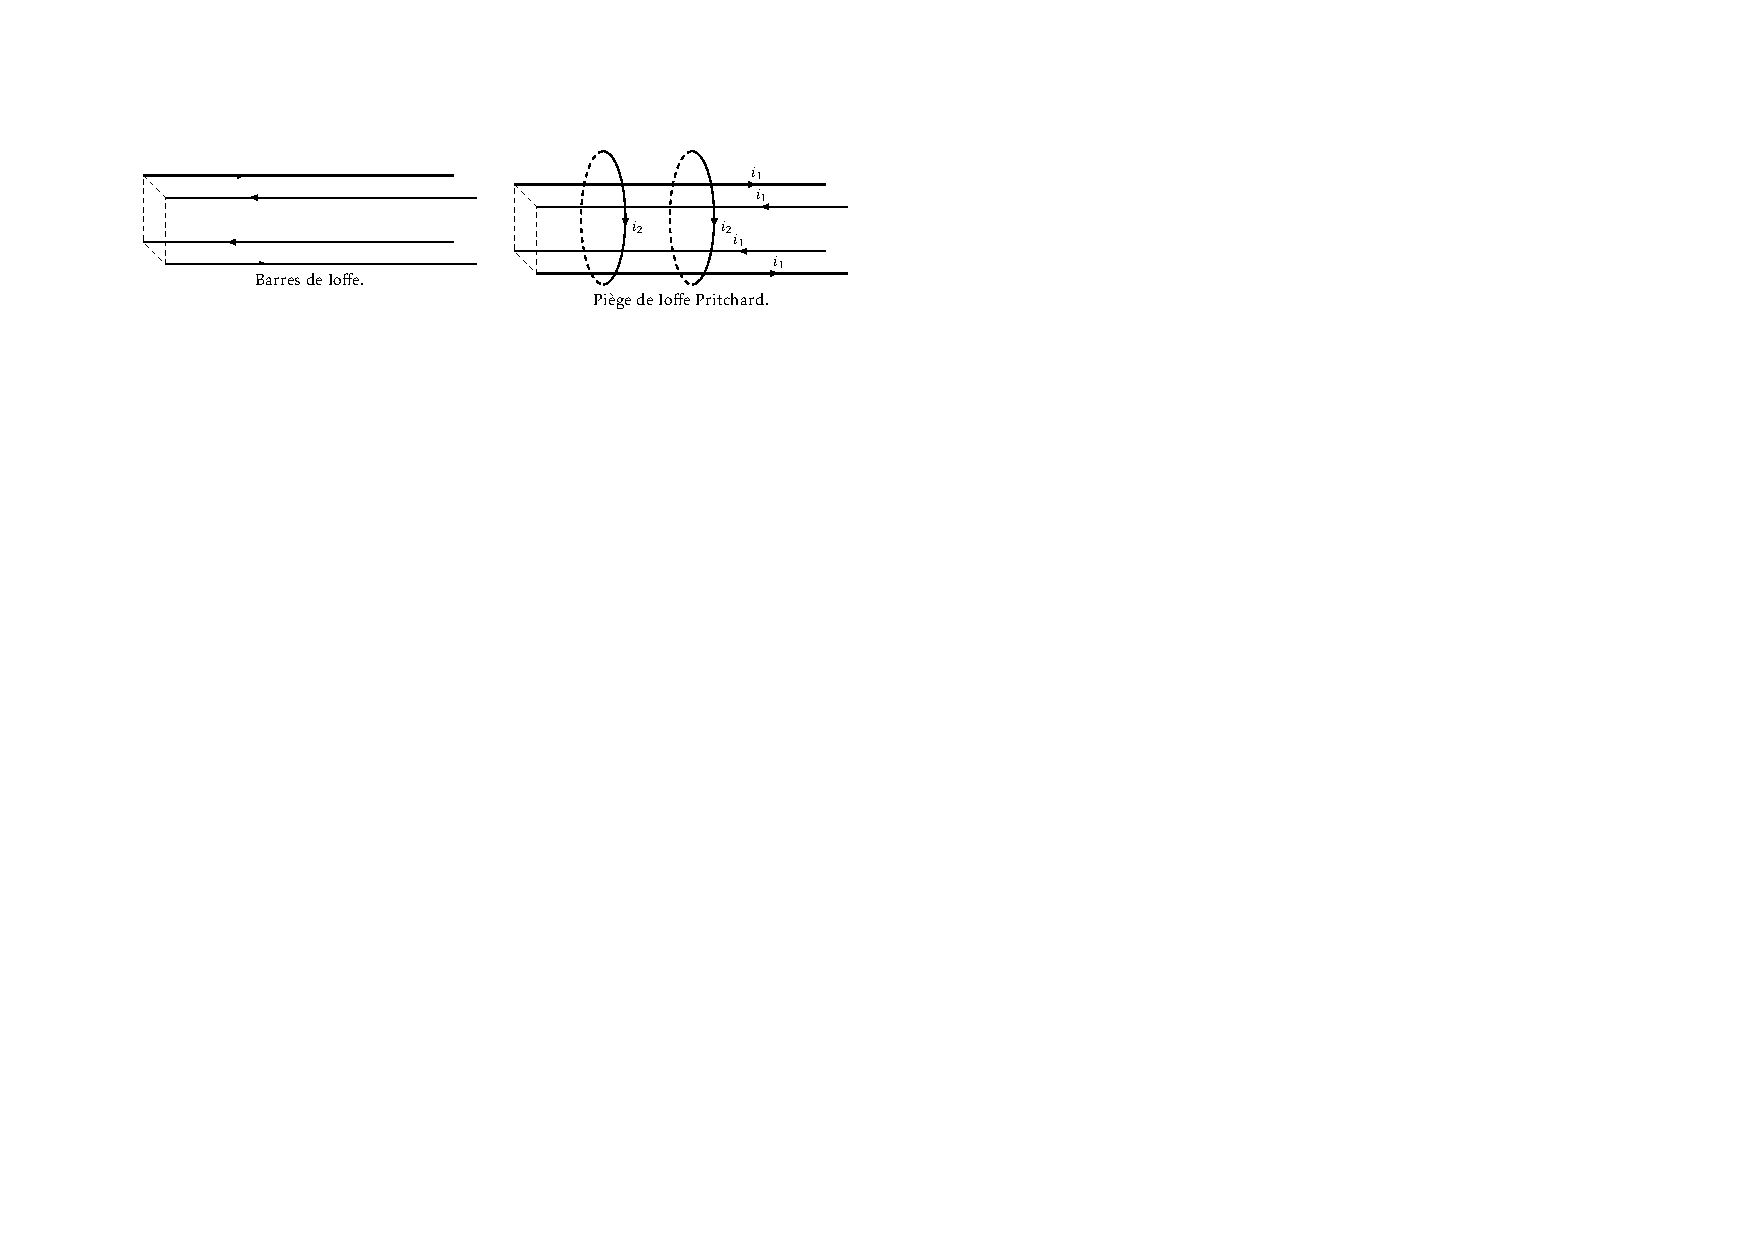
\includegraphics[width=\linewidth]{oraux/mines/Ioffe.pdf}  
\end{center}

\begin{questions}
    \questioncours Redémontrer rapidement l'expression du champ magnétique $b_1$ émis par un fil infini parcouru par un courant $i_1$ le long de l'axe $\ve_z$.
    \question Montrer qu'il peut s'exprimer sous la forme
    $$\vec{b}_1(\vr) = \rot\vec{a}_1 \qqtext{avec} \vec{a}_1(\vr) = a_0\ln (r/r_0)\ve_z,$$
    avec $\vec{a}_1$ un champ qu'on appelle le potentiel vecteur du champ magnétique et $a_0$ une constante dont on donnera l'expression et $r_0$ une constante arbitraire. \vspace{-1em}
    \uplevel{
    \paragraph{Attention :} le potentiel vecteur est une notion hors programme ; il ne sera pas exigé du ou de la candiat$\cdot$e de connaissance à son sujet. On s'en tiendra à la seule définition mathématique $\vB = \rot\vA$.}
    \uplevel{On s'intéresse maintenant au champ magnétique $B_1$ émis par les barres de Ioffe : quatre fils identiques disposés en carré de côté $c$, comme dans la figure ci-dessus. On note $xy$ le plan du carré et $x=0$, $y=0$ le centre du carré. On note $r$ la distance au centre du carré dans le plan $xy$.}
    \question Sans calcul donner l'allure des lignes de champ $B$ dans le plan $xy$. Quelle est la valeur du champ au centre du carré ?
    \question On se place proche de $r=0$ en considérant que $r\ll c$. Calculer le potentiel vecteur du champ magnétique $A_1$ des barres de Ioffe en $\vr$. On prendra la constante $r_0 = c$.
    \question En déduire l'expression pour le champ $B_1$.
    \uplevel{Afin de contraindre également la particule dans la direction des $z$, on ajoute deux spires de rayon $R$ séparées d'une distance $d$ : c'est le piège de Ioffe--Pritchard.}
    \question 
    Le champ magnétique $b_2$ émis par une seule spire de courant $i_2$ si on se place sur son axe de révolution est
    $$b_2(z) = \dfrac{\mu_0 i_2 R^2}{2(R^2+z^2)^{3/2}}.$$
    Au vu de vos connaissances sur les symétries du champs magnétique et sur les dipôles magnétiques, interpréter cette expression.
    \question En supposant que l'on soit proche du milieu des deux spires et sur leur axe de révolution, calculer le champ magnétique $B_2$ émis par les deux spires.
    \question Lorsqu'on somme $B_1$ et $B_2$, quel type de profil de champs magnétique a-t-on ? Interpréter en terme de trajectoire d'une particule chargée proche du centre.
\end{questions}

\paragraph{Données} $\rot$ est l'opérateur rotationnel dont l'expression en coordonnées cylindriques est
$$\rot\vec{a} = \qty(\dfrac{1}{r}\pdv{a_z}{\theta} - \pdv{a_\theta}{z})\ve_r +\qty(\pdv{a_r}{z} - \pdv{a_z}{r})\ve_\theta + \dfrac{1}{r}\qty(\pdv{(ra_\theta)}{r} - \pdv{a_r}{\theta})\ve_z$$

\end{exercise}


\section{X--ENS}
\begin{exercise}{Gaz quantique d'électrons}{-1}{Spé}
{Quantique,Boltzmann}{lelay}

On considère un puits infini unidimensionnel de taille $L$ dans lequel se trouve un gaz parfait de $N$ particules quantiques de masse $m$.

\begin{questions}
    \question \textbf{Cas $N = 1$ :} Donner les énergies accessibles $\varepsilon_n$, en fonction de $m$, $L$, la constante de Planck $h$ et $n\in\mbb{N}^\ast$ un entier. \\
    Quelle est l'énergie minimale $\varepsilon^\ast$ de cette particule ?
    \question \textbf{Cas $N > 1$ :} Rappeler la définition d'un gaz parfait. En déduire que l'énergie totale du système est
    $$\En = \varepsilon^\ast\sum_{i=1}^{N} n_i^2, \qquad n_i\in\mbb{N}^\ast.$$
    \uplevel{On suppose que le gaz est à l'équilibre à la température $T$.}
    \question Donner la probabilité que l'énergie du système soit égale à $\En$ en fonction de $\beta = \frac{1}{k_\textsc{b}T}$ et d'une constante de normalisation $\cal{Z}(\beta)$ dont on donnera l'expression sous forme d'une somme.
    
    \question Exprimer l'expression de l'énergie moyenne du système $U$ du système. Montrer que
    $$U = -\pdv{\ln\cal{Z}}{\beta}.$$
    
    \question Montrer qu'en supposant la taille du système $L$ très grande devant une longueur $\Lambda$ que l'on précisera, on peut approximer la somme $\cal{Z}(\beta)$ sous la forme continue suivante :
    $$\cal{Z} = \qty(\dfrac{L}{\Lambda})^{N}\times \underset{1}{\underbrace{\dfrac{1}{\pi^{N}}\int_{\mbb{R}^{N}} e^{-\norm{\vec{x}}^2} \dd[N]{\vec{x}}}} = \qty(\dfrac{L}{\Lambda})^{N}.$$
    
    \uplevel{Si les particules quantiques considérées sont des fermions (par exemple, des électrons), il ne peut y avoir deux particules coexistant dans le même état.}
    
    \question Quel est le nom de ce principe dans le cas des électrons ? Peut-on encore supposer le gaz parfait ?
    
    \question Montrer qu'il faut donc modifier l'expression précédente sous la forme
    $$\cal{Z} = \qty(\dfrac{L}{\Lambda})^{N}\times \dfrac{1}{\pi^{N}}\int_{\mbb{R}^{N}} e^{-\norm{\vec{x}}^2} f(\vx) \dd[N]{\vec{x}},$$
    où on précisera l'expression de $f$.
    
    \question Cas $N=2$. Exprimez $\cal{Z}$. On pourra considérer, puisque les particules sont indiscernables, que $n_1 < n_2$.
    
    On pourra s'aider des intégrales gaussiennes suivantes :
    $$\forall k\in\mbb{N}^\ast : \int_0^y \text{Erf }^{k-1}(x) e^{- x^2}\dd{x} = \dfrac{\sqrt{\pi}}{2k}\text{Erf }^k(y), \qqtext{et} \lim_{y\rightarrow\infty}\text{Erf }^k(y) = 1.$$
    
    \question Généralisation pour $N$ ?

    
\end{questions}

\end{exercise}